%!TeX spellcheck = en-GB

%Basics
\documentclass[aps, prb, a4paper, english, 12pt, onecolumn, longbibliography, amsmath, amssymb, colorinlistoftodos, floatfix, svgnames]{revtex4-2}
\usepackage[utf8]{inputenc}
\usepackage{babel}

%Symbols and scientifics
\usepackage{amsmath, amsfonts, amssymb, bm}
\numberwithin{equation}{subsection}
\usepackage{physics}
\usepackage{mathtools}
\usepackage{siunitx}
\sisetup{
	per-mode = power ,
	round-mode = figures ,
	round-precision = 3 ,
	scientific-notation = false ,
	output-decimal-marker = {.} ,
	exponent-product = \times ,
	separate-uncertainty = true ,
	uncertainty-separator = \ ,
	output-product = \cdot ,
	quotient-mode = fraction ,
	range-phrase = - ,
	range-units =  single ,
	inter-unit-product = \ensuremath{{\cdot{}}} ,
	number-unit-product = \ ,
	multi-part-units = single ,
	alsoload = synchem ,
	alsoload = addn
}
\DeclareSIUnit\atm{atm}
\usepackage{chemfig}
\usepackage{tikzorbital}

%Appendix, TOC and Bibliography
\usepackage{appendix}
\renewcommand\appendixtocname{Appendices}
%\usepackage[nottoc]{tocbibind}
\usepackage[lastpage,user]{zref}

%Figures
\usepackage{float}
\usepackage{xcolor} % Required to specify font color
\usepackage{graphicx}
\usepackage{subcaption}
\usepackage[format=plain,
            labelfont={bf,it},
            textfont=it]{caption}
\usepackage[verbose]{wrapfig}
\usepackage[a4paper, centering, rmargin=2.5cm, tmargin=2.5cm, lmargin=2.5cm, bmargin=2.5cm]{geometry}
\usepackage{etoolbox}
\usepackage{verbatim}
\usepackage[space]{grffile}
\usepackage[final]{pdfpages}
\usepackage{array}
\usepackage{multirow}
\usepackage{dcolumn}
%\usepackage{animate}
\usepackage{fontawesome}
\usepackage[european]{circuitikz}
\usepackage{pdflscape}
\usepackage{pgfplots}
\pgfplotsset{width=10cm, compat=newest}
\def\axisdefaultwidth{10cm}
%\usepgfplotslibrary{external}
\usepgfplotslibrary{units}
%\tikzexternalize
\usepackage{pgfgantt}
\newcounter{myWeekNum}
\stepcounter{myWeekNum}
%
\newcommand{\myWeek}{\themyWeekNum
    \stepcounter{myWeekNum}
    \ifnum\themyWeekNum=53
         \setcounter{myWeekNum}{1}
    \else\fi
}
%

%Header footer
\usepackage{fancyhdr}
\pagestyle{fancy}
\lhead{C. V. Sørensen \\ R. K. F. Wiuff}
\chead{Quantum Transport in NPG\\DTU Department of Physics}
\rhead{May \nth{1}\\2019}
\cfoot{Page \thepage\, of \zpageref{LastPage}}
\renewcommand{\headrulewidth}{0.4pt}
\renewcommand{\footrulewidth}{0.4pt}

%Text tools
\usepackage{listings}
\usepackage{parcolumns}
\usepackage[super]{nth}
\usepackage[normalem]{ulem}
\usepackage{import}
\usepackage{url}
\usepackage{lipsum}
\usepackage{microtype}
\usepackage[pdfencoding=auto, psdextra]{hyperref}
\hypersetup{
	colorlinks   = true, %Colours links instead of ugly boxes
	urlcolor     = blue, %Colour for external hyperlinks
	linkcolor    = blue, %Colour of internal links
	citecolor   = red %Colour of citations
}
\usepackage[capitalise]{cleveref}
\usepackage{enumitem}
\setlist[enumerate]{itemsep=0mm}
\usepackage{booktabs}
\usepackage{silence}
\usepackage{todonotes}
\WarningFilter{revtex4-2}{Repair the float package.}

%Python
\usepackage{minted}
\setminted{fontsize=\small}
\usemintedstyle{monokai}
\renewcommand{\listoflistingscaption}{Listings}
%\renewcommand{\MintedPygmentize}{C:/Users/rwiuf/AppData/Roaming/Python/Python37/Scripts/pygmentize}
\newcommand{\im}[3]{\inputminted[bgcolor=Black, linenos=true, python3=true, firstline=#2, lastline=#3]{python}{#1}}

%Definitions and new commands
\newcommand{\degr}{^{\circ}}
\newcommand{\me}{\mathrm{e}}
\newcommand*\mathinhead[2]{\texorpdfstring{$\boldsymbol{#1}$}{#2}}
%PDFPages and RevTeX incompatability fix
\makeatletter
\AtBeginDocument{\let\LS@rot\@undefined}
\makeatother

\begin{document}
%Titlepage herunder:
\begin{abstract}
	\vspace{5mm}
	\centering
	\begin{description}
		\item[Abstract] Abstract... \vspace{3\baselineskip}
	\end{description}
	
\includegraphics[width=1cm]{Figures/DTU3CMYK.eps}
\end{abstract}

\title{Quantum Transport in Nanoporous Graphene}
\date{May \nth{1} 2019}
\author{Rasmus Kronborg Finnemann Wiuff (s163977)}
\email[E-mail at ]{rwiuff@dtu.dk}
\author{Christoffer Vendelbo Sørensen (163965)}
\email[E-mail at ]{chves@dtu.dk}
\affiliation{Technical University of Denmark}
\homepage[Homepage of the Technical University of Denmark ]{http://www.dtu.dk/english/}
\homepage[\\\faGithub \ Project Repository: ]{https://github.com/rwiuff/QuantumTransport}
\maketitle

\pagenumbering{arabic}
\twocolumngrid
\tableofcontents
\onecolumngrid

% ToC before List-ofs fix
\makeatletter
\let\toc@pre\relax
\let\toc@post\relax
\makeatother

\thispagestyle{empty}
%\newpage
\setcounter{page}{1}

%Text
\section{Introduction}
%!TEX root = ../Main.tex
\lipsum{5}\cite{calogero_electron_2019}
\subsection{Pi-orbitals and Basis sets }
\section{Quantum transport}
%!TEX root = ../Main.tex
In this section, the basics of the tight-binding approximation for electron transport will be explained. This motivates the use of numerical routines using NumPy.
\subsection{Ballistic quantum transport}
As graphene is a two dimensional material that consists of carbon atoms arranged in a hexagonal pattern, features in such a material can approach nanometer and sub nanometer scales. Because of the small scale the electrical properties of the material is vastly different from normal materials. Usually when describing the electrical properties of a material, drift-diffusion current models are used. They describe electric charges per area and current per area. This is usually a good description in systems where electron-electron and electron-atom scatterubg frequently occurs. The distance an electron travels before such a event is called its \textit{mean free path}. However, in small systems as those of NPG-devices, the mean free path is longer than the system itself. Experiments have shown that electrons can move ballistically in graphene and carbon nanotubes[litt], that is, without phonon scattering. Therefore, we model electron transport using the \textit{ballistic model}. In this model the electrons move through the material as waves. The fact that the electrons moves as waves will prove important later on because it gives rise to \textit{Quantum Interference} which can be exploited as a tool when engineering graphene-based devices. Furthermore the model looks at only one electron at a time in the presence of an electron gas. This model has been used with big success for regular graphene and it seems that the ballistic model also gives a good approximation for NPGs.
\subsection{\mathinhead{\pi}{\pi}-orbitals and \mathinhead{\pi}{\pi}-electrons}
When modelling the electron transport in graphene one needs to address the orbital structure of carbon lattices. The orbital structure is exactly what motivate the use of tight binding approximation and Green's functions. The two concepts of Tight-binding approximation and Green's functions will be elaborated further in the coming sections.
In its basic form graphene can be divided into rings of carbon atoms as shown in \cref{ring}. In the (\(x,y\))-plane the carbon atoms are bound in \(sp^2\) orbitals as shown in \cref{sp2}.
\begin{figure}[ht]
    \centering
    \begin{subfigure}[b]{0.3\textwidth}
	    \begin{tikzpicture}
		    \chemfig{C*6(-C-C-C-C-C-)}
	    \end{tikzpicture}
	    \caption{Graphene lattices consists of hexagonal arrangements of carbon atoms.}\label{ring}
    \end{subfigure}
    ~
    \begin{subfigure}[b]{0.3\textwidth}
	\centering
	\resizebox{\textwidth}{!}{
		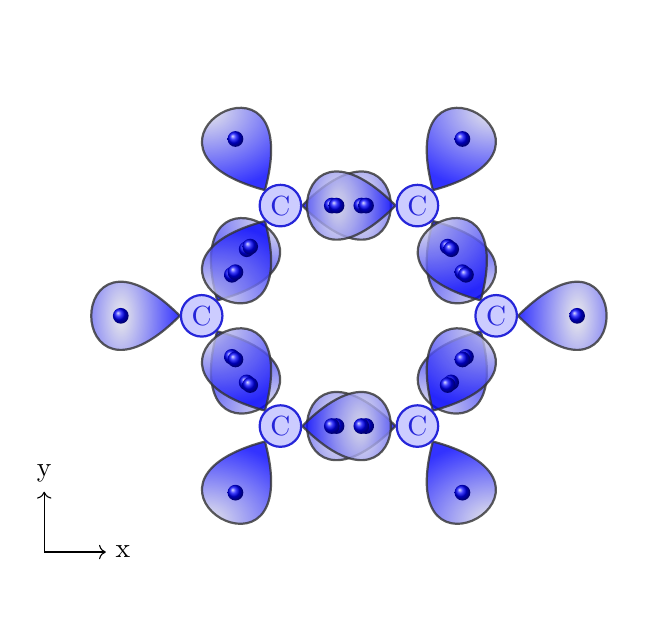
\begin{tikzpicture}
		    \node (x) at (-1,-3) {x};
		    \node (y) at (-2,-2) {y};
		    \draw[->] (-2,-3) -- (x);
		    \draw[->] (-2,-3) -- (y);
			\satom[name=C, color=blue, pos={(0,0)}]{
				blue/60/north east/2/1,
				blue/180/west/1,
				blue/300/south east/2/1
			}
			\satom[name=C, color=blue, pos={(1,1.4)}]{
				blue/0/east/2/1,
				blue/120/north west/1,
				blue/240/south west/2/1
			}
			\satom[name=C, color=blue, pos={(2.74,1.4)}]{
				blue/60/north east/1,
				blue/180/west/2/1,
				blue/300/south east/2/1
			}
			\satom[name=C, color=blue, pos={(3.74,0)}]{
				blue/0/east/1,
				blue/120/north west/2/1,
				blue/240/south west/2/1
			}
			\satom[name=C, color=blue, pos={(2.74,-1.4)}]{
				blue/60/north east/2/1,
				blue/180/west/2/1,
				blue/300/south east/1
			}
			\satom[name=C, color=blue, pos={(1,-1.4)}]{
				blue/0/east/2/1,
				blue/120/north west/2/1,
				blue/240/south west/1
			}
		\end{tikzpicture}}
	\caption{Carbon atoms in a hexagonal lattice are \(sp^2\) hybridised in the (\(x,y\))-plane.}\label{sp2}
    \end{subfigure}
    \caption{Benzene ring and its \(sp^2\) hybradised orbitals.}\label{Benz}
\end{figure}
This hybridisation lock all but one valence electron for the carbon atoms. These electrons exists in a p-orbital in the \(z\)-direction.
\cref{p} shows the valence orbitals of carbon.
\begin{figure}[H]
	\begin{center}
		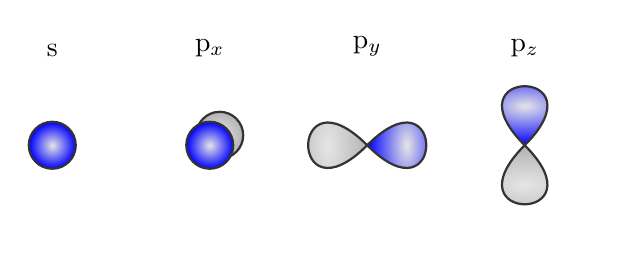
\begin{tikzpicture}
			\orbital[pos = {(0,3)}] {s}
			\node[above] at (0,4) {s};
			\orbital[pos = {(2,3)}]{px}
			\node[above] at (2,4) {p$_x$};
			\orbital[pos = {(4,3)}]{py}
			\node[above] at (4,4) {p$_y$};
			\orbital[pos = {(6,3)}]{pz}
			\node[above] at (6,4) {p$_z$};
		\end{tikzpicture}
		\caption{The valence orbitals of carbon.}
		\label{p}
	\end{center}
\end{figure}
The last electron in the p\(_z\) orbital does not mix with the tightly bound s, p\(_x\) and p\(_y\) electrons and moves freely. Thus these electrons have higher energies compared to the \(sp^2\) electrons and occupy states at the Fermi level. These electrons dominates transport in the graphene lattice. The p\(_z\) orbital is also known as the \(\pi\)-orbital and as such the electron lying there is called a \(\pi\)-electron. Through a carbon lattice the \(\pi\)-electrons will travel through \(\pi\)-orbitals. For a benzene ring the \(\pi\)-electrons at the highest occupied molecular state will travel through the p\(_\pi\)-orbitals switching sign as they travel as shown in \cref{sign}.
\begin{figure}[H]
	\begin{center}
		\pgfdeclarelayer{background}
		\pgfdeclarelayer{middle}
		\pgfdeclarelayer{foreground}
		\pgfsetlayers{background,middle,main,foreground}
		\begin{tikzpicture}
			\begin{pgfonlayer}{background}
				\orbital[pos = {(6,6)}]{-pz}
				\node[above] at (6,7) {-p$_\pi$};
				\orbital[pos = {(4,6)}]{pz}
				\node[above] at (4,7) {p$_\pi$};
				\draw[dashed, very thick] (6,6) -- (4,6);
				\draw[dashed, very thick] (7,4.73) -- (6,6);
				\draw[dashed, very thick] (4,6) -- (3,4.73);
			\end{pgfonlayer}
			\orbital[pos = {(7,4.73)}]{pz}
			\node[above] at (7,5.73) {p$_\pi$};
			\orbital[pos = {(3,4.73)}]{-pz}
			\node[above] at (3,5.73) {-p$_\pi$};
			\begin{pgfonlayer}{foreground}
				\orbital[pos = {(4,3.46)}]{pz}
				\node[above] at (4,4.46) {p$_\pi$};
				\orbital[pos = {(6,3.46)}]{-pz}
				\node[above] at (6,4.46) {-p$_\pi$};
				\draw[dashed, very thick] (4,3.46) -- (6,3.46);
			\end{pgfonlayer}
			\draw[dashed, very thick] (6,3.46) -- (7,4.73);
			\draw[dashed, very thick] (3,4.73) -- (4,3.46);
		\end{tikzpicture}
		\caption{When jumping from one carbon atom to another, the \(\pi\)-electron goes between p\(_\pi\)-orbitals. Such a jump is described by two matrix elements in the system's Hamiltonian.}
		\label{sign}
	\end{center}
\end{figure}
\subsection{Tight-binding}\label{tbtheory}
Now that the transport carrying electrons are defined the next step is describing the transport itself. For this purpose we employ the \textit{tight-binding} approximation. In this approximation the electrons are considered being tightly bound to the atoms. Contrary to a free electron gas approximation, the electrons does not spend time in between orbitals, but jump from orbital in atom \(a\) to orbital in atom \(b\). The Hamiltonian is represented as a matrix of hopping elements for a collection of neighbouring atomic orbitals, i.e. molecular orbitals, as well as the energy contained within each orbital (which will be addressed later on). This can be done by describing the orbitals as a Linear Combination of Atomic Orbitals (LCAO). The solution to the Schrödinger equation is then:
\begin{align}
	\Psi_{\mathrm{MO}} = \sum_{\alpha,R}c_{\alpha,R}\phi_{\alpha}(R)
\end{align}
where \(\phi_{\alpha}(R)\) is an atomic orbital at position \(R\), with \(\alpha\) denoting the valence of the orbital (\(2s,2p_x,2p_y,2p_z\)). In electron transport the states close to the Fermi level is of interest. These are namely the highest occupied molecular orbitals (HOMO), or the lowest unoccupied molecular orbitals (LUMO). As stated earlier only the \(\pi\)-electrons is then of interest.
The electrons' motion can be described with the hopping matrix of elements:
\begin{align}
	V_{pp\pi} = \bra{\phi_{\pi}(1)}\hat{H}\ket{\phi_{\pi}(2)}\label{V}
\end{align}
Physically this means that there is a potential between the \(\pi\) orbitals of neighbouring atoms \(1\) and \(2\). In our tight-binding approximation we consider only hop between nearest neighbours. The element
\begin{align}
	\epsilon_0 = \bra{\phi_{\pi}(1)}\hat{H}\ket{\phi_{\pi}(1)}
\end{align}
is the average energy of the electron on atom \(1\) and, it is common to define the hopping energy relative to this, i.e. \(\epsilon_0 = 0\).
If the atoms or their environment differs, so does the on-site potential.\newline
\cref{benzex} contains an illuminating example of how the tight-binding approximation can be used to describe simple carbon systems.
\section{Band structure of NPG}
%!TEX root = ../Main.tex
\subsection{Creating on-site Hamiltonian and hopping matrices for the system}
In order to calculate and visualise the band structure of the NPG within a unit cell, the on-site Hamiltonian along with its hopping matrices must be defined. The on-site Hamiltonian lies within the unit cell of the system. As the unit cell is repeated periodically the on-site Hamiltonian fills out one full period of the system. The unit cell is defined with respect given unit vectors which determine the periodicity of the system. By these definitions the elements of the hopping matrices represents hops between the repeated unit cells with respect to the periodicity. See \cref{atomrepfig} for a visual representation of the structure with its periodicity. \\
On the premise of the Tight Binding Model, the next step to find all the nearest neighbouring atoms within the given set of atom coordinates to define the on-site Hamiltonian \(\bf{h}_0\) and then define the hopping matrices \(\bf{V}\) and its conjugate \(\bf{V}^{\dagger}\). This is because the Tight Binding model only allow for hopping of electrons between nearest neighbours which in this case is the periodic boundary conditions set for the system.\\ \textit{Maybe implement code pieces or explain code terms that executes these operations. i.e. "By using two for loops and the numpy function np.subtract(), we get the all the combinations of... etc. This should be considered throughout the section.} This can be done simply by taking what is similar to an outer product of the coordinate matrix with itself only here every combination of coordinates are subtracted not multiplied, hereafter taking the norm of all those combinations. This will produce a matrix which contain all distances between all atoms in the NPG. Once obtained a threshold will be applied to sort out the nearest neighbours within the matrix. In this specific case the coordinates given was with respect to unit vectors with a lattice constant of \(\SI{1.0}{\angstrom}\), which means that the threshold in this case should be \(\SI{1.6}{\angstrom}\) which is the inter-atomic distance for nearest neighbours in a graphene mesh. All distances above \(\SI{1.6}{\angstrom}\) will be changed to a 0-element in the on-site Hamiltonian as no hopping of electrons is possible between atoms that are more than one inter-atomic distance apart. All distances below the threshold will be changed to 1 to represent a hop between to atoms. The on-site Hamiltonian is then multiplied by at scalar which is the on-site potential \(V_{ppi}\) which in this case is \(-1\). Now the on-site Hamiltonian is complete and the construction of the hopping matrices can begin. \\
As the on-site Hamiltonian represents a (three)two-dimensional structure one has to make sure that hopping between the nearest neighbour atoms relative to that of a repeated unit cell (on-site Hamiltonians) can described in all directions in the plane. Effectively this means that six hopping matrices should be created. One in the x-direction, one in the y-direction, one in the xy-direction and their hermitian conjugates. Graphically this corresponds to a structure of this kind:
\begin{figure}[H]
    \centering
    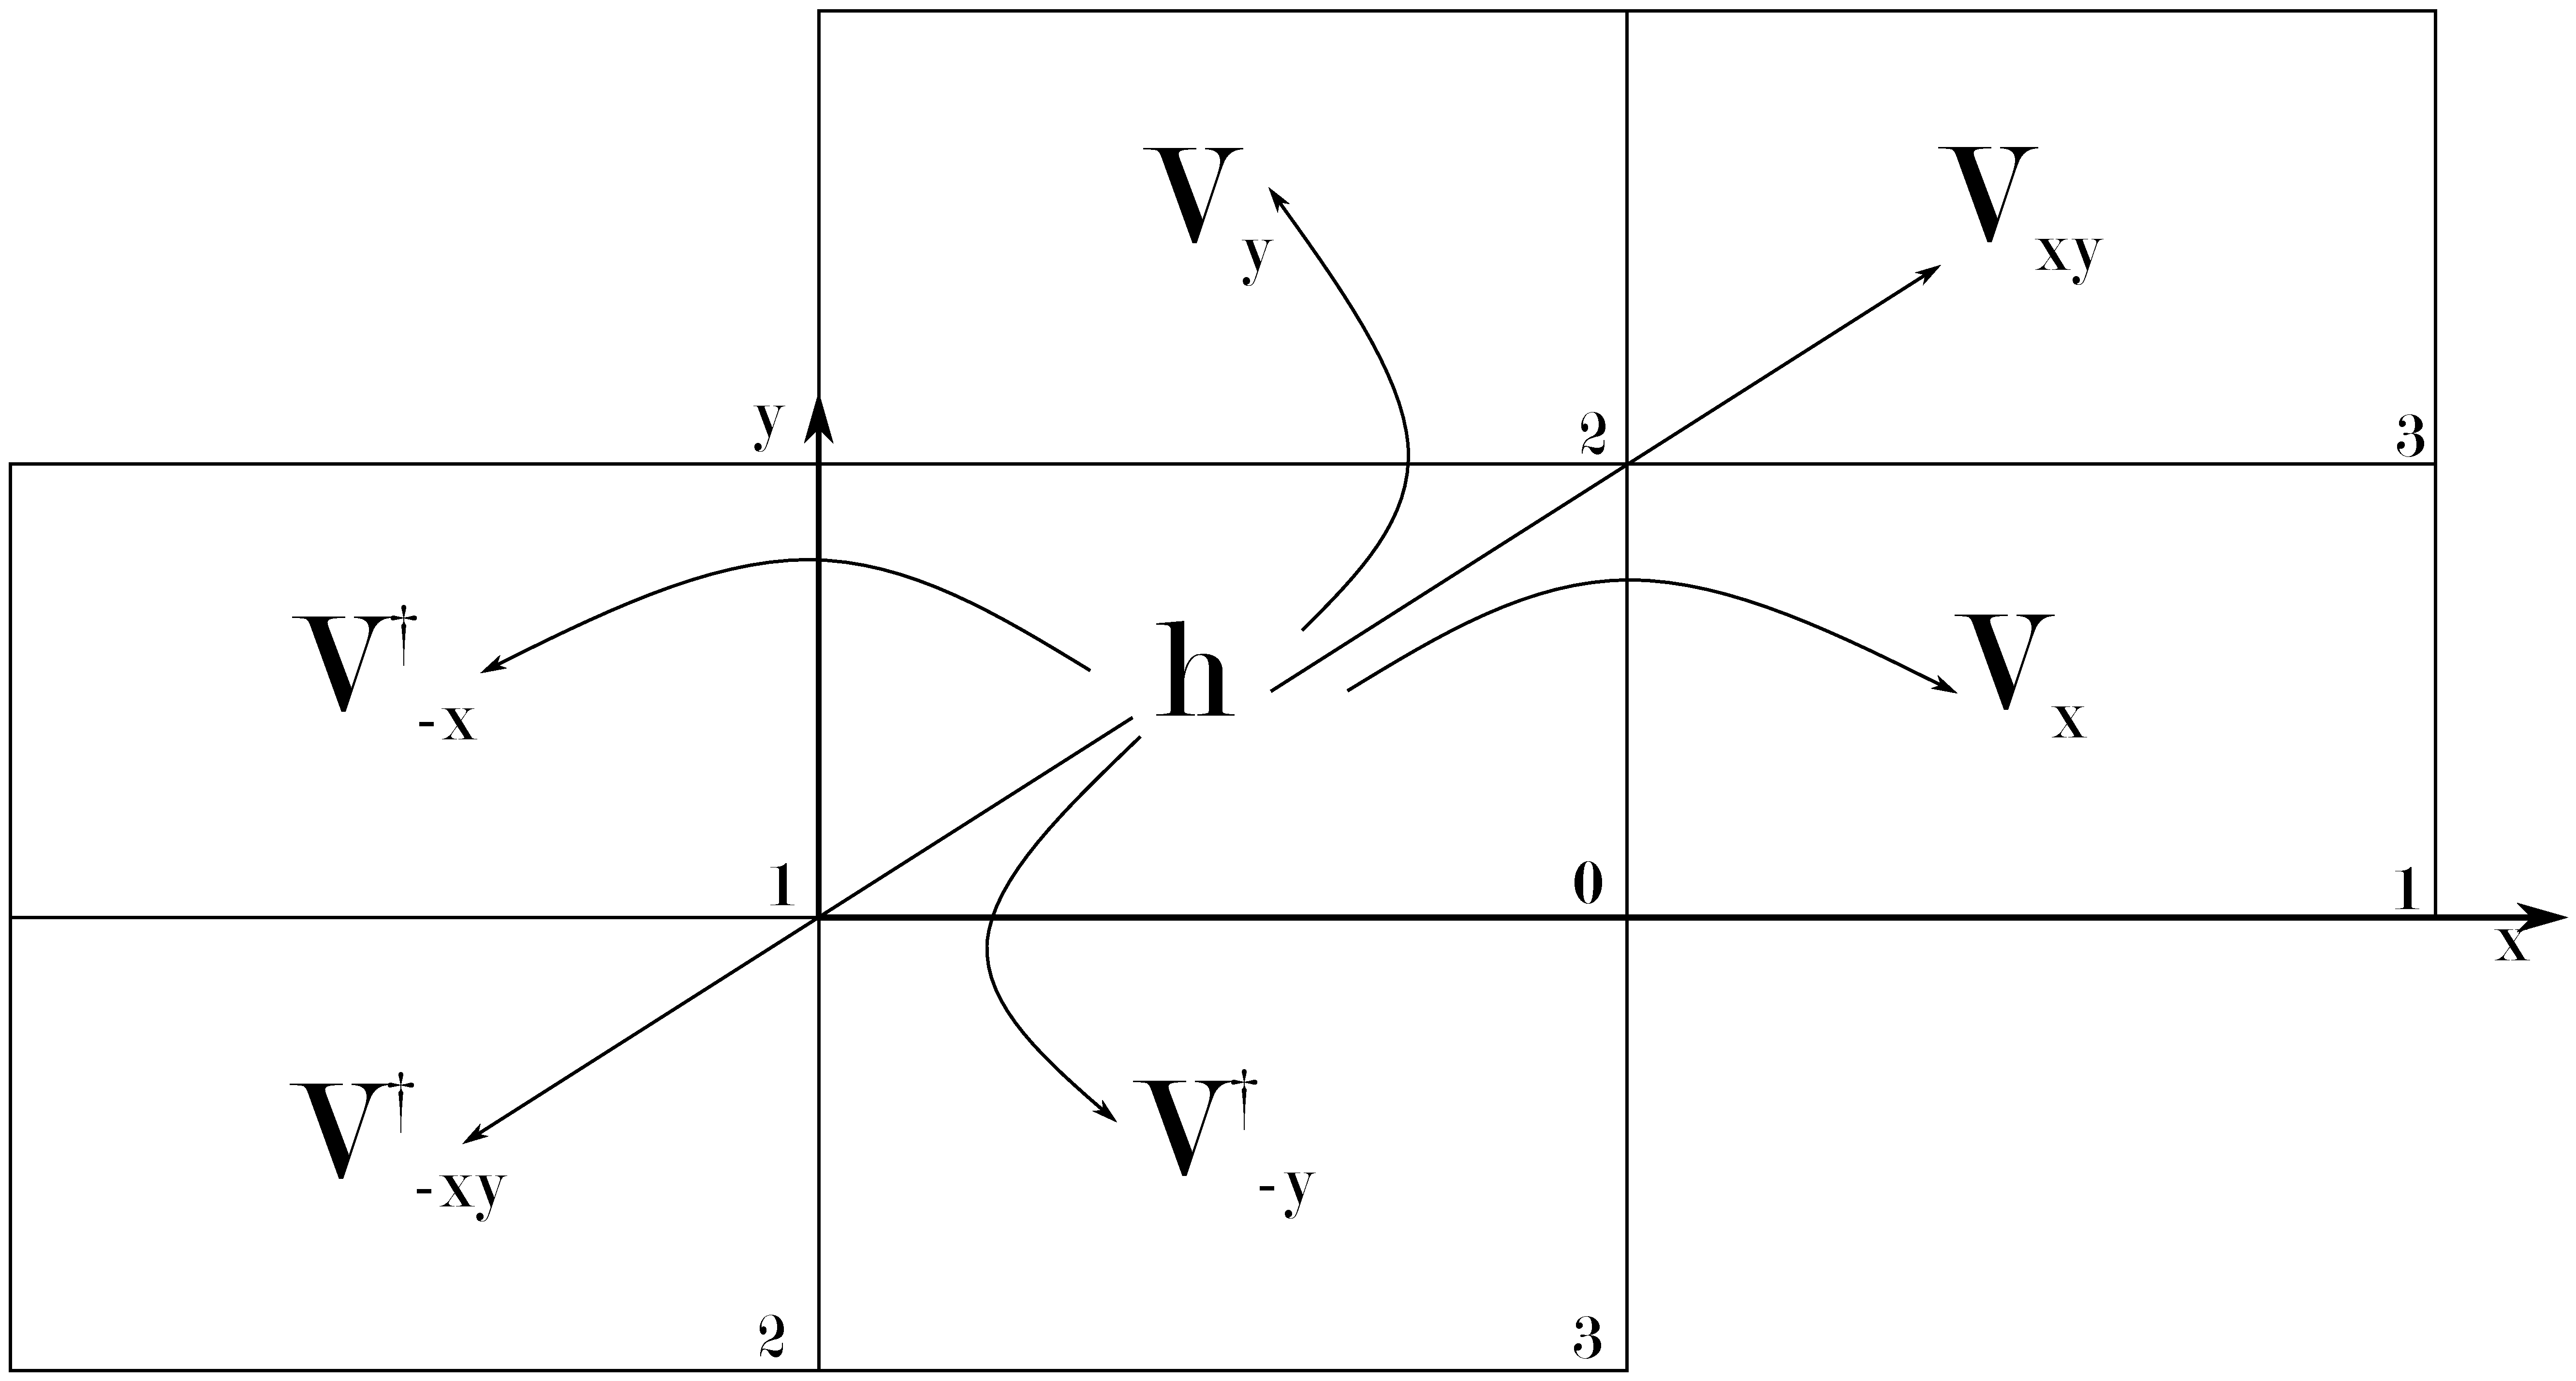
\includegraphics[width = 0.7\textwidth]{Figures/repfig.eps}
    \caption{Representative figure of how the on-site Hamiltonian along with its hopping matrices are structured}
    \label{repfig}
\end{figure}
In practice this is done by shifting the original coordinates by the given unit vectors of the system in each direction, adding the unit vector to the coordinate matrix making three new matrices. Now that three shifted matrices has been obtained, the same routine to find the distances as with the on-site Hamiltonian can be utilised, the only difference being that the outer subtraction will be between the on-site Hamiltonian and the shifted matrices respectively to make sure it is the distance between the on site Hamiltonian and the shifted matrices that is calculated. Again by replacing the distances in the shifted matrices with 1 and 0 according to the inter-atomic threshold, the hopping matrices are obtained. The three hopping matrices denoted \(\vb{V}_{1x}\), \(\vb{V}_{2y}\) and \(\vb{V}_{3xy}\) represent hopping in the "forward" direction (left-to-right). To create the hopping matrices hopping in the "backwards" (right-to-left) direction one simply has to transpose the hopping matrices. These matrices are denoted with a dagger: \(\vb{V}_{1x}^{\dagger}\), \(\vb{V}_{2y}^{\dagger}\) and \(\vb{V}_{3xy}^{\dagger}\). \cref{matrixmap} is a figure of the resulting matrix-maps from the calculation, stitched together like in \cref{repfig}.

\begin{figure}[H]
    \centering
    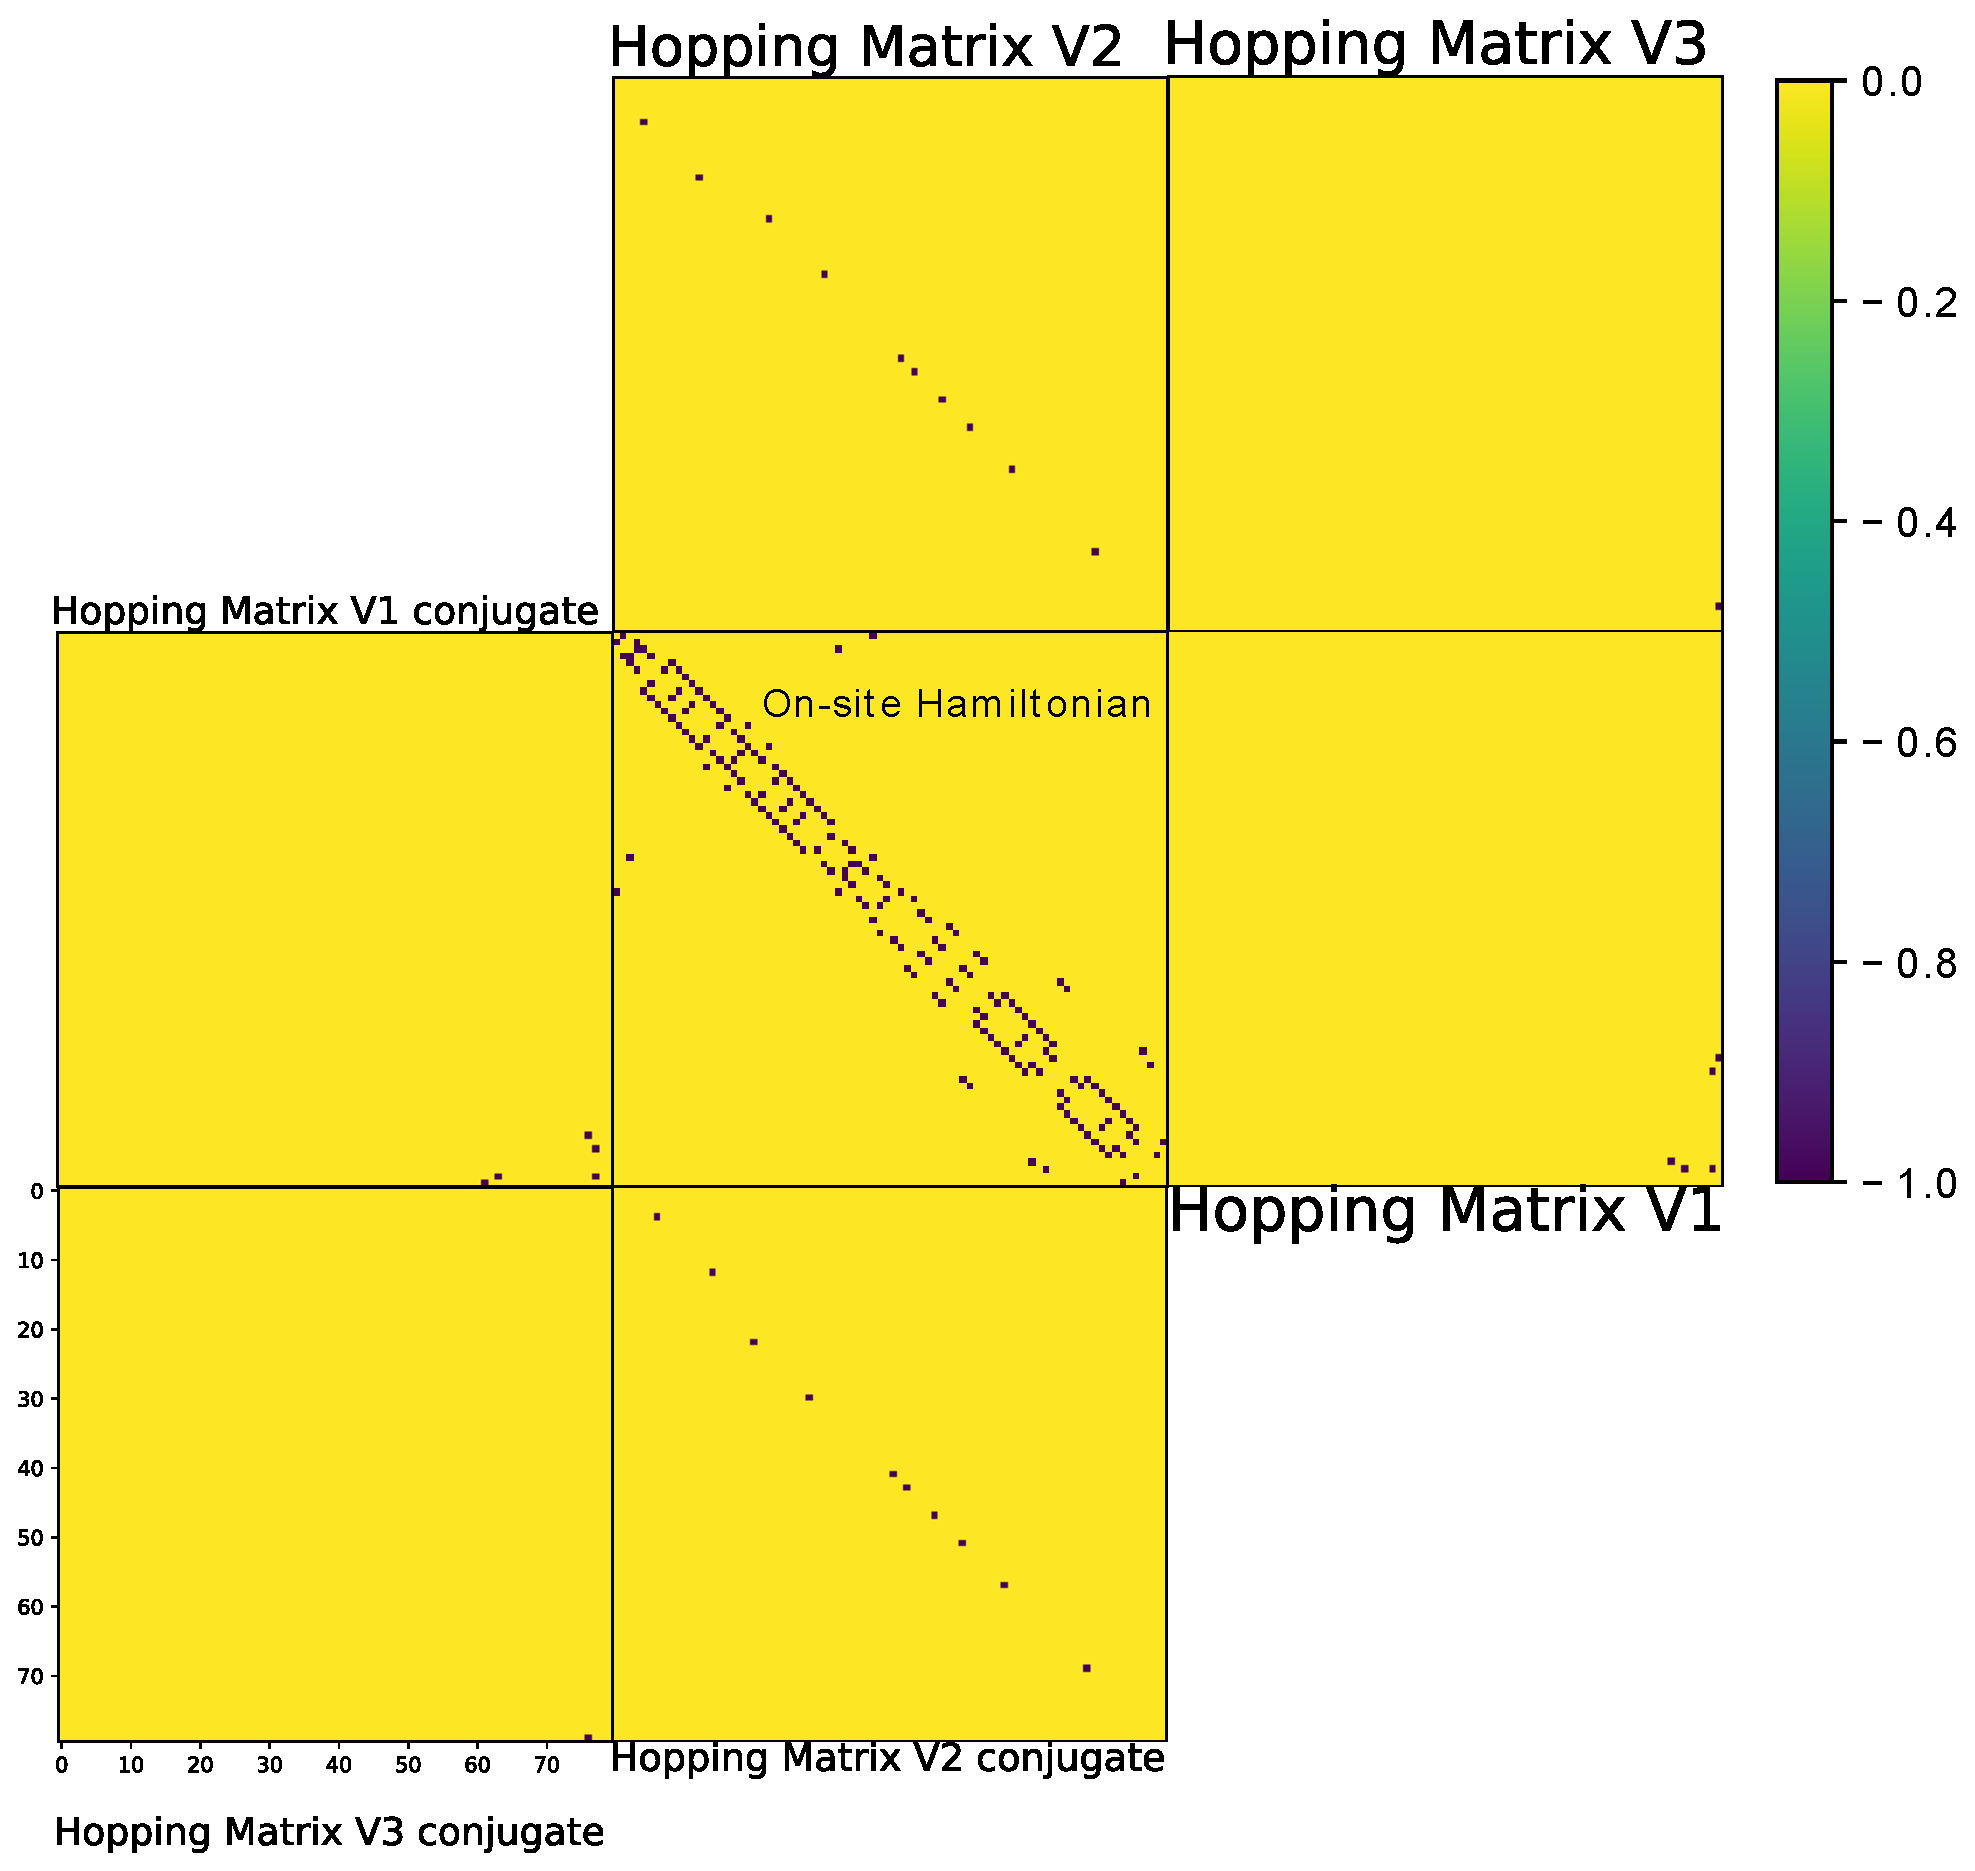
\includegraphics[width=\textwidth]{Figures/Matrixmap.eps}
    \caption{Matrix maps from calculation on the NPG. The on-site Hamiltonian along with all its hopping matrices are stitched together like the representative figure \cref{repfig}. All the dark spots represents a hopping of an electron to its nearest neighbour.}
    \label{matrixmap}
\end{figure}
\begin{figure}[H]
    \centering
    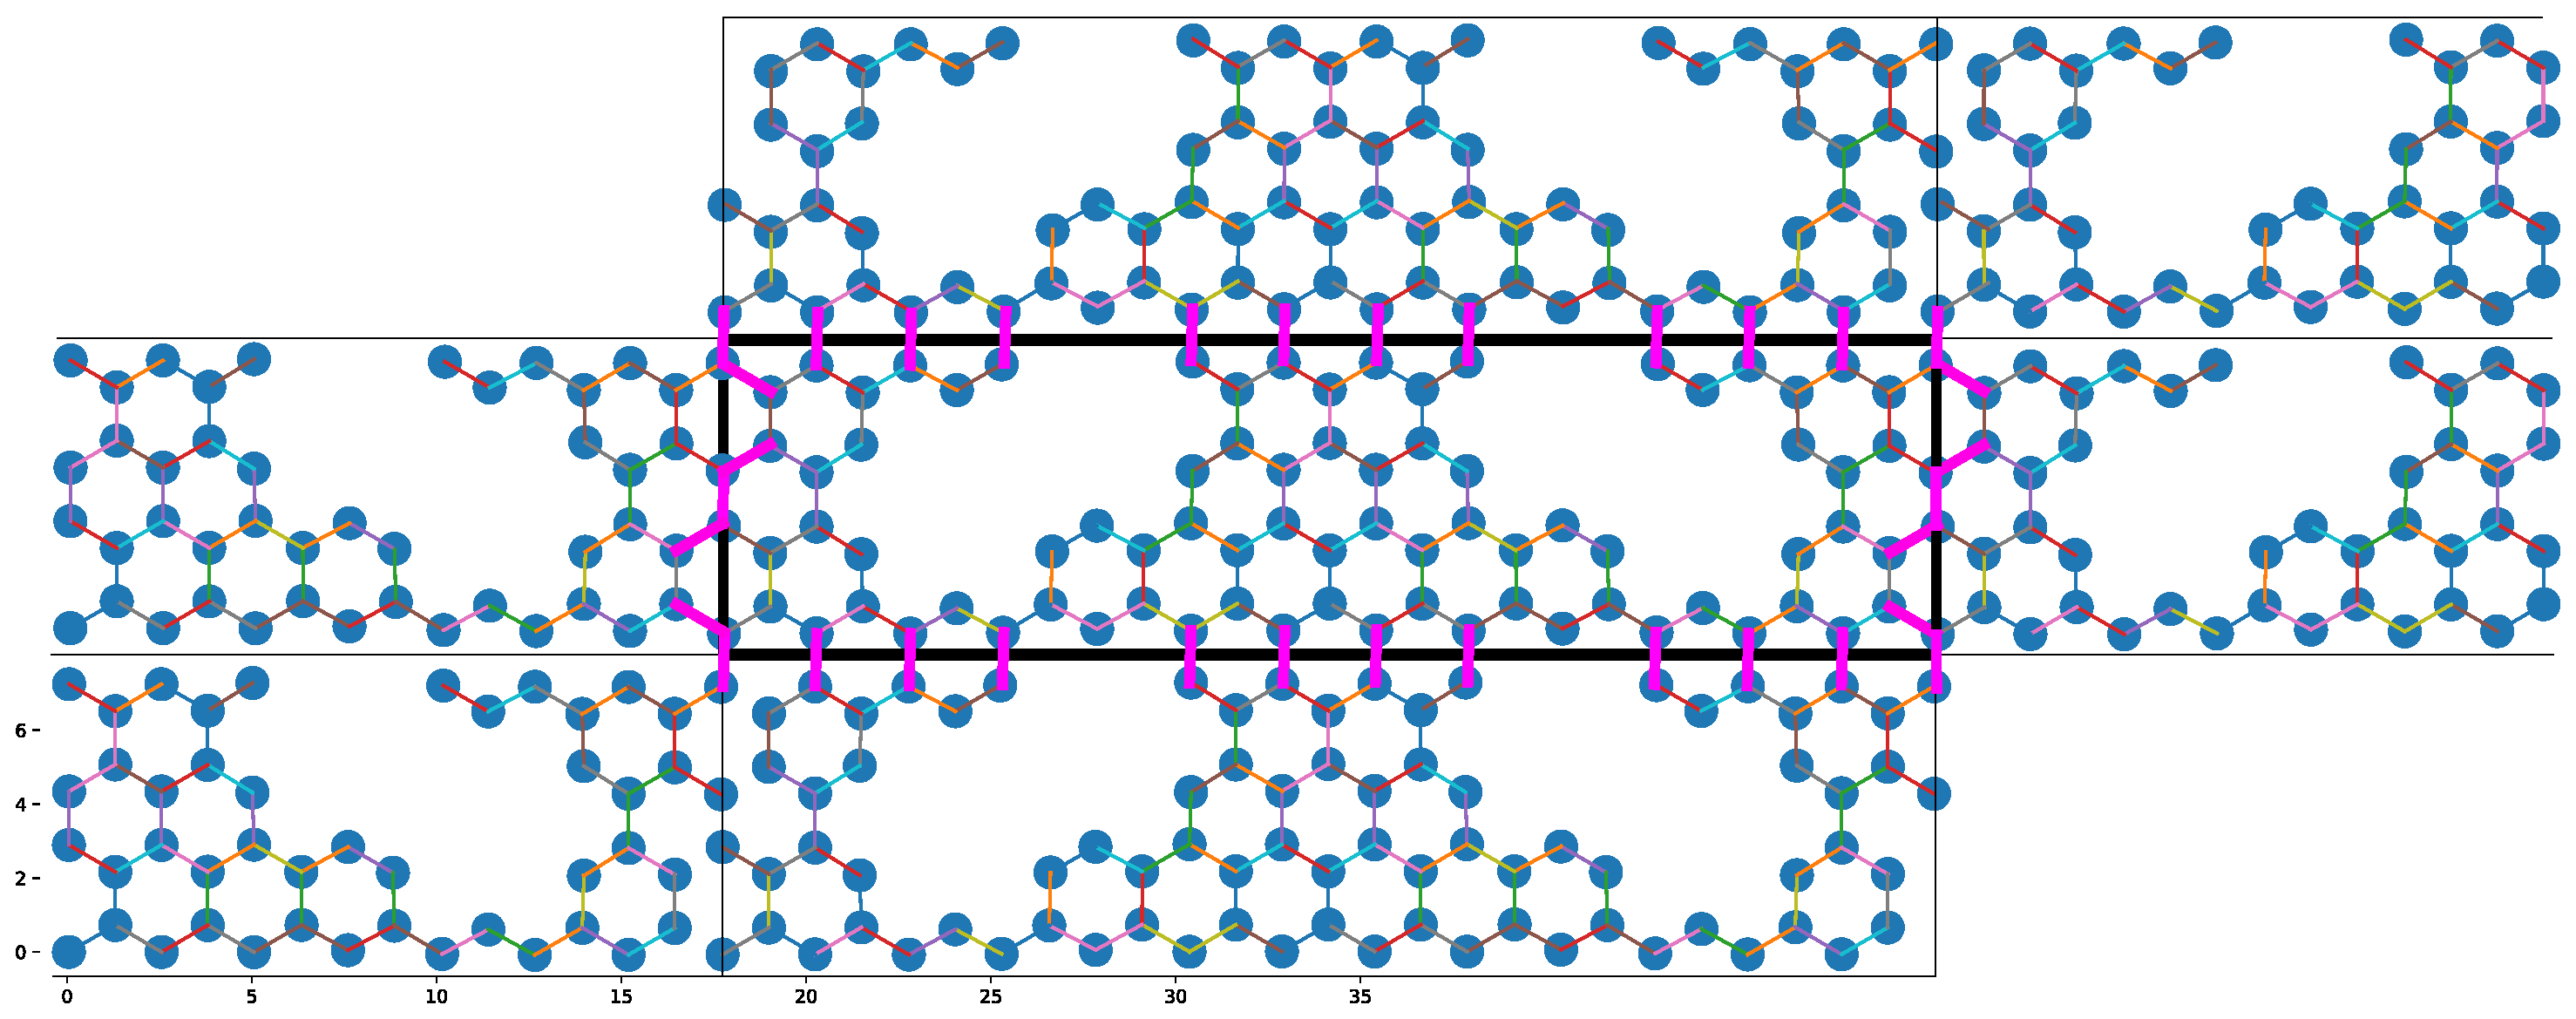
\includegraphics[width=\textwidth]{Figures/representativestructure2.eps}
    \caption{Visual representation of the periodic NPG-structure. The atoms surrounded by the black box in the centre represents the unit cell. The neighbouring boxes are unit cells repeated periodically. Note that the two cells left and right with respect to the centre cell has been cut in half for figure space. The pink lines crossing the black box represents the link between the nearest neighbours in the adjacent cell. Note how this representation corresponds to that of \cref{matrixmap}. There is more 'hopping' when going up and down, than left or right and the two cells at the diagonal only have one atom which is nearest neighbour to the centre cell which corresponds to the one hopping elements in \cref{matrixmap}.}
    \label{atomrepfig}
\end{figure}
\subsection{Defining the full Hamiltonian and solving the Schrodinger equation}\label{FullHam}
Now that the on-site Hamiltonian along with its hopping matrices has been defined, the next step is to create the full Hamiltonian in order to solve the Schrodinger equation for system, which is a eigen-value/vector problem. In essence the full Hamiltonian denoted \(\vb{H}\) is a sum of the on-site Hamiltonian and its corresponding hopping matrices multiplied by a complex exponential function that has the appropriate phase relative to the hopping matrix:
\begin{flalign}\label{\hamileq}
\begin{split}
\vb{H}(k_x,k_y) = &\vb{h}_0 + (\vb{V}_{1x}e^{-ik_x} + \vb{V}_{1x}^{\dagger}e^{ik_x} + \vb{V}_{2x}e^{-ik_y} + \vb{V}_{2x}^{\dagger}e^{-ik_y}\\ & + \vb{V}_{3xy}e^{-ik_x}e^{-ik_y} + \vb{V}_{3xy}^{\dagger}e^{ik_x}e^{ik_y})
\end{split}
\end{flalign}
Here \(k\) represents a continuous variable between 0 and \(\pi\) along the x- and y-axis in inverse space.
Using the full Hamiltonian, the Schrodinger equation can be solved
\begin{align}
    \vb{H}(k_x,k_y)\vb*{\phi}_{k} = \vb*{\epsilon}_n (k_x,k_y) \vb*{\phi}_k
\end{align}
In practice this is all done by defining a function that takes the on-site Hamiltonian, the hopping matrices, and \(k\) as inputs and outputs the eigenvalues, using numpy's \textit{numpy.linalg.eigh}. The number of eigenvalues in the output corresponds to the dimension of the full Hamiltonian. In \cref{fullhamil} the code for the function is shown.\begin{listing}[ht]
    \centering
    \im{Listings/Functions.py}{51}{60}
    \caption{Function producing the full hamiltonian, corresponding to \cref{\hamileq}}
    \label{fullhamil}
\end{listing}As the eigenvalues corresponds to the eigenenergies of the system, the band structures can be plotted.
\subsection{Plotting the band structures}
The continuous variable \(k\) extends in two directions (\(-k_{x}\)) and (\(k_{y}\)) which corresponds to lengths between the symmetry points \(X\), \(\Gamma\) and \(Z\) in the Brillouin zone, with \(\Gamma\) being the zero-point. It is therefore necessary to make two plots, one for each pair of symmetry points. The y-values in each plot corresponds to the eigenvalues obtained by the function described in \cref{FullHam}. Each x-value between \(\Gamma\), \(X\) and \(\Gamma\), \(Z\) therefore has associated with it the amount of y-values which the dimension of full Hamiltonian dictates. F.ex. if the full Hamiltonian has dimension \(80\times80\) there is 80 eigenvalues associated with it and the amount of y-values for each x-value between \(\Gamma\), \(X\) and \(\Gamma\), \(Z\) is 80. In this specific case, the full Hamiltonian for obtaining the eigenvalues that corresponds to \(X\) and \(Z\) are:
\begin{align}\label{hamilxgamma}
X: \ \vb{H}_{X} = \vb{h}_0 + (\vb{V}_{1x}e^{ik_x} + \vb{V}_{1x}^{\dagger}e^{-ik_x} + \vb{V}_{2x} + \vb{V}_{2x}^{\dagger} + \vb{V}_{3xy}e^{ik_x} + \vb{V}_{3xy}^{\dagger}e^{-ik_x})\\
Z: \ \vb{H}_{Z} = \vb{h}_0 + (\vb{V}_{1x} + \vb{V}_{1x}^{\dagger} + \vb{V}_{2x}e^{-ik_y} + \vb{V}_{2x}^{\dagger}e^{ik_y} + \vb{V}_{3xy}e^{-ik_y} + \vb{V}_{3xy}^{\dagger}e^{ik_y})
\end{align}
Using the eigenvalues as y-values in the two plots, putting the two plots together  will yield a full plot of the band structure shown in \cref{Fab}.
\begin{figure}[H]
    \centering
    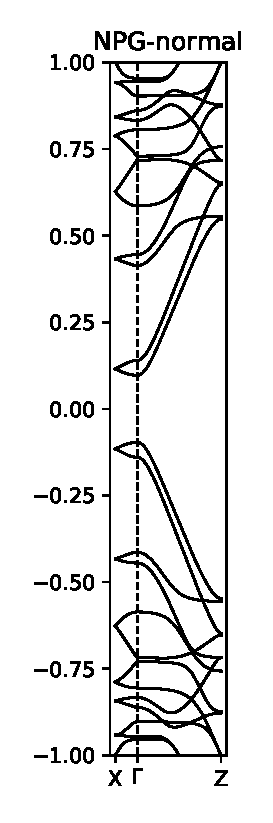
\includegraphics{Figures/FabNPGBS.eps}
    \caption{Plot showing the band structure in the energy range -1 to 1 for NPG with normal bridges between symmetry points \(X\) and \(Z\) with respect to \(\Gamma\)}
    \label{Fab}
\end{figure}

\begin{figure}
    \centering
    \begin{subfigure}[b]{0.3\textwidth}
        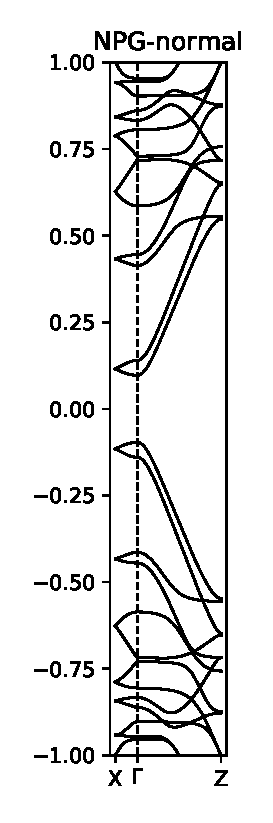
\includegraphics[width=\textwidth]{Figures/FabNPGBS.eps}
                \caption{Plot showing the band structure in the energy range -1 to 1 for NPG with normal bridges between symmetry points \(X\) and \(Z\) with respect to \(\Gamma\)}
        \label{Fabbs}
    \end{subfigure}
    ~ %add desired spacing between images, e. g. ~, \quad, \qquad, \hfill etc.
      %(or a blank line to force the subfigure onto a new line)
    \begin{subfigure}[b]{0.3\textwidth}
        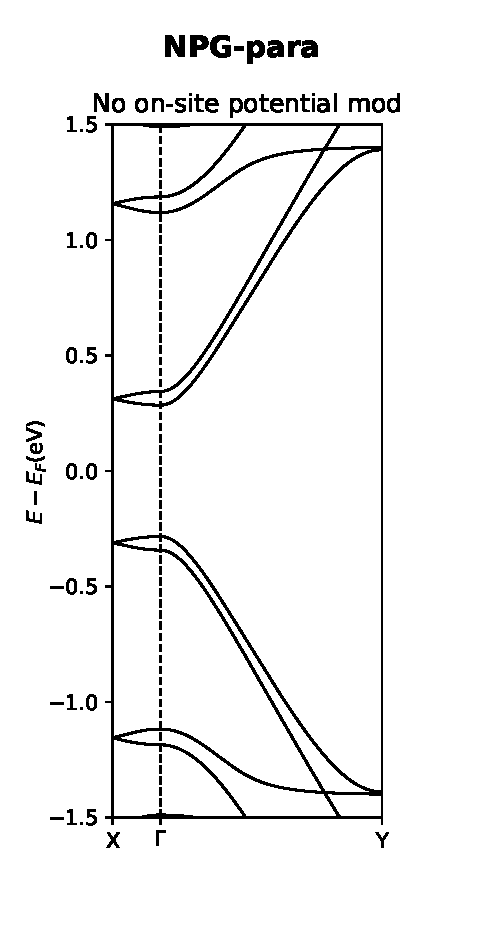
\includegraphics[width=\textwidth]{Figures/paraNPGBS.eps}
        \caption{Plot showing the band structure in the energy range -1 to 1 for NPG with para bridges between symmetry points \(X\) and \(Z\) with respect to \(\Gamma\)}
        \label{parabs}
    \end{subfigure}
    ~ %add desired spacing between images, e. g. ~, \quad, \qquad, \hfill etc.
    %(or a blank line to force the subfigure onto a new line)
    \begin{subfigure}[b]{0.3\textwidth}
        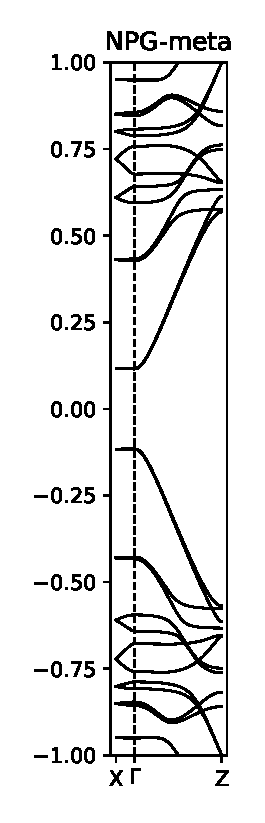
\includegraphics[width=\textwidth]{Figures/metaNPGBS.eps}
        \caption{Plot showing the band structure in the energy range -1 to 1 for NPG with meta bridges between symmetry points \(X\) and \(Z\) with respect to \(\Gamma\)}
        \label{metabs}
    \end{subfigure}
    \caption{Figure showing para, meta and normal NPG band structures}\label{allbands}
\end{figure}

\section{Self Energy, Greens Functions and the Recursion Routine}
%!TEX root = ../Main.tex
The Green's function and self energies play the central role when it comes to obtaining the LDOS as well as electron transport in a system. In fact, the imaginary part of the Green's function is the LDOS for a specific site in a system. What the Green's function and self energy actually is and how they come about will here be explained formally, to motivate the practical use in the following sections.\subsection{Green's functions and self-energy}\label{greensandself}
Some of the concepts in this section will be explained using  the simle system as an example (\cref{atomrepfig}). However, in the following section (\cref{recursionroutinesec}) the focus will revert back to the simple system from \cref{pointplot}. \begin{figure}[H]
	\centering
	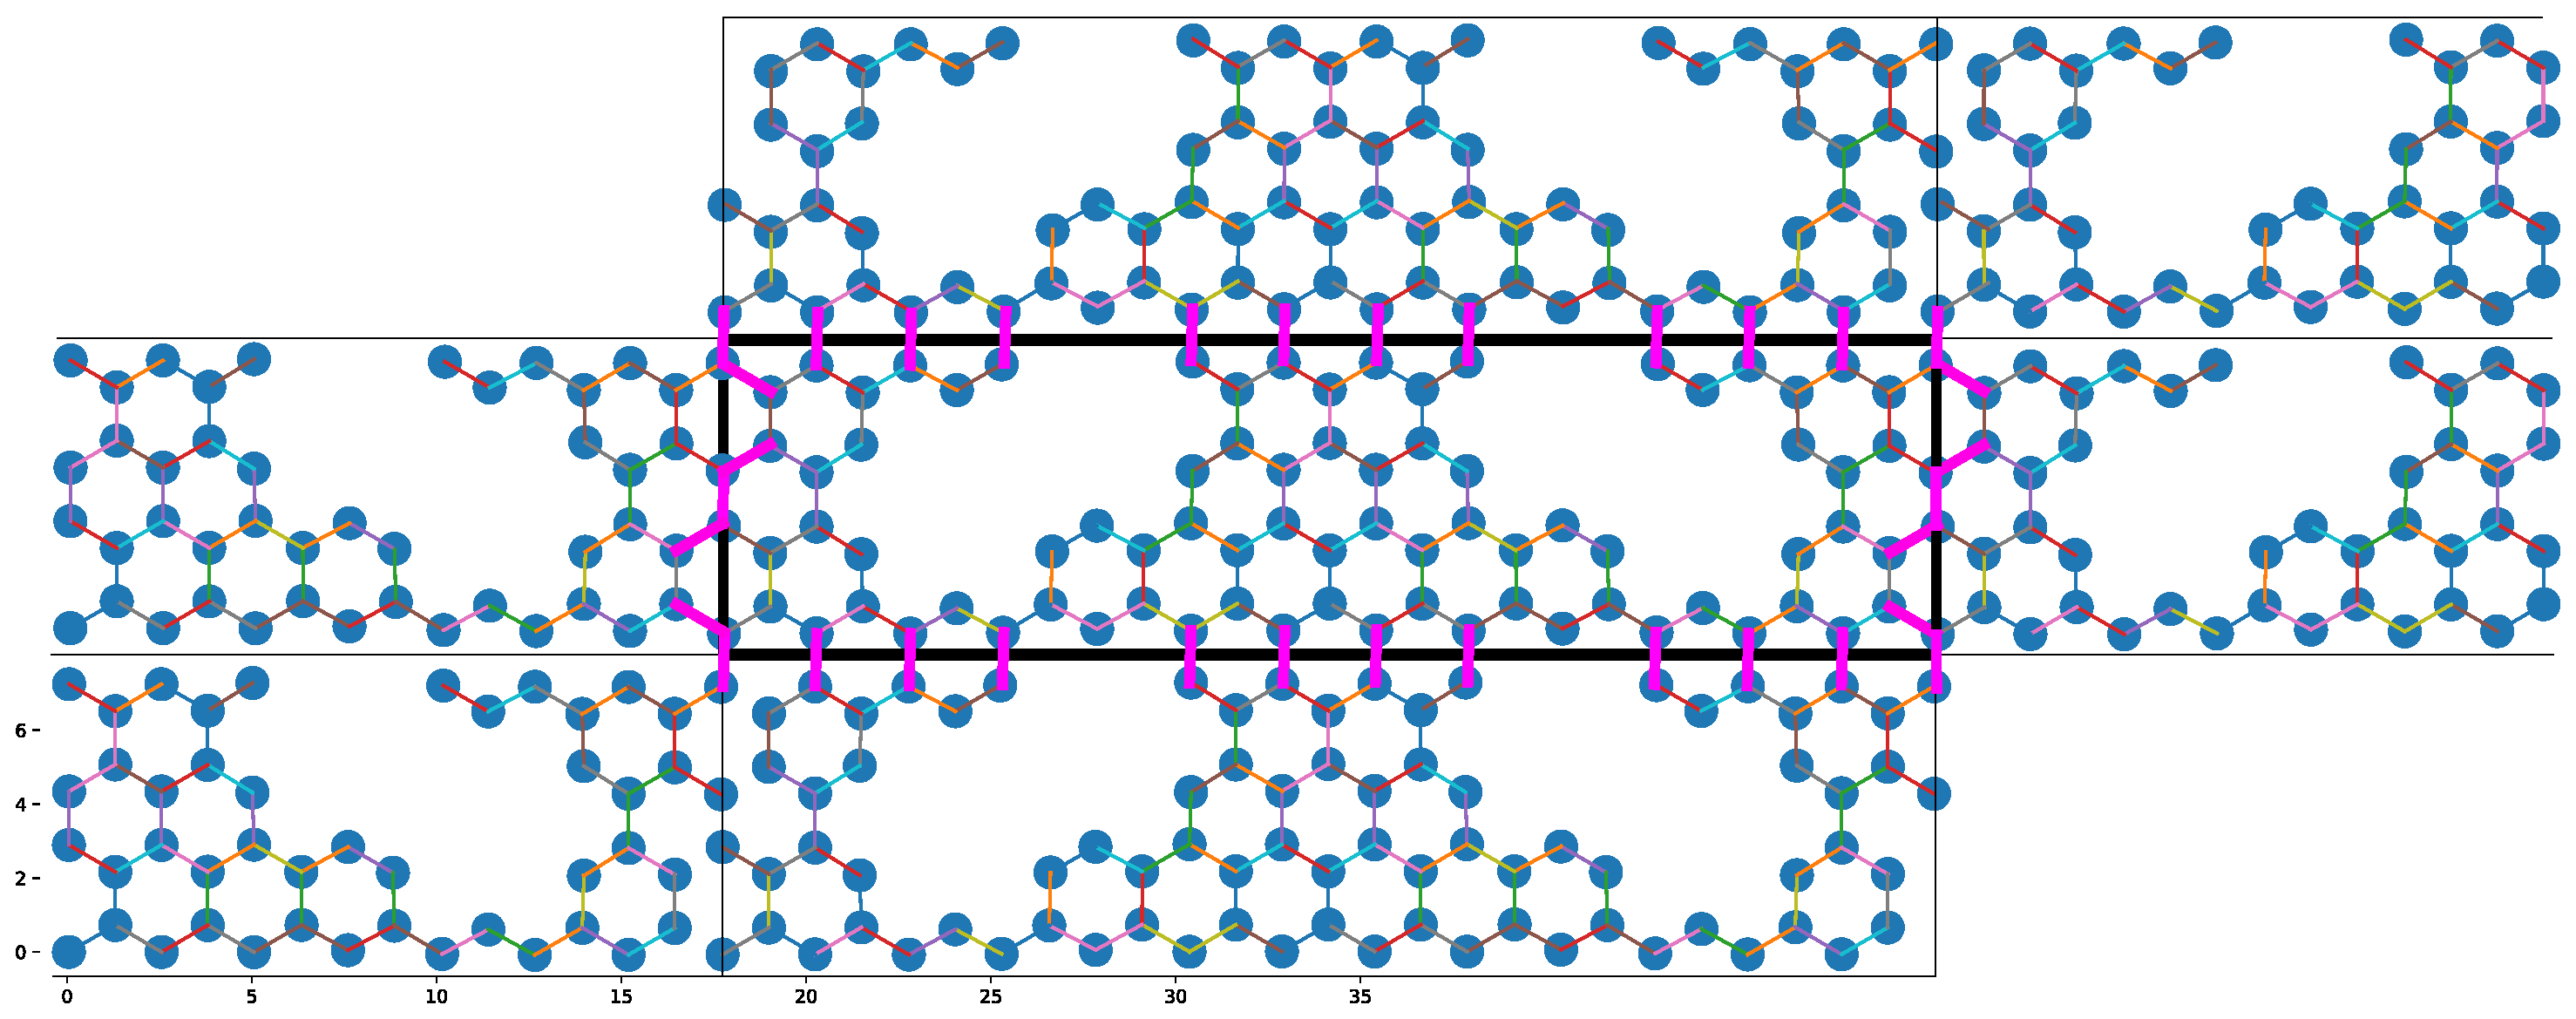
\includegraphics[width=\textwidth]{Figures/representativestructure2.eps}
	\caption{Visual representation of the periodic NPG-structure. The atoms surrounded by the black box in the centre represents the unit cell. The neighbouring boxes are unit cells repeated periodically. Note that the two cells left and right with respect to the centre cell has been cut in half for figure space. The pink lines crossing the black box represents the link between the nearest neighbours in the adjacent cell.}
	\label{atomrepfig}
\end{figure}
%\begin{align}
%\mathbf{H}\phi(t) &= i\pdv{t}\phi(t) \\
%\mathbf{H}\mathbf{G}(t) &= i\pdv{t}\mathbf{G}(t)
%\end{align}
%with specific boundary conditions, namely\begin{align}\label{boundary}
%    \phi(t=0) = f
%\end{align}
%The Green's function has the additional property that \(\mathbf{G}(t=0)=\mathbf{1}\) which means the one can solve the TDSE for any initial value of \(t\)  if one has solved the equation for the Green's function first.\begin{align}\label{greenssolution}
%    \phi(t)=\mathbf{G}(t)f
%\end{align}
%From \cref{greenssolution} it can be seen that the Green's function propagates the value \(f\) at \(t=0\). Now, if the Hamiltonian is time independent one can also consider time independent solutions to the Schr\"{o}dinger Equation. All states will then be oscillating with the same complex phase, at a specific energy \(E\). This will be given by \(e^{-iEt}\).
Imagine a system like the one in \cref{atomrepfig}. It contains a unit cell in the centre, marked by a black border, surrounded by repeated unit cells in all directions. The aim is to explain how electrons move through this region. Suppose all cells surrounding the centre cell are considered "contacts" in the sense that they represent a semi-infinite chain of molecules and that they are the source of electrons (or states) that is injected in to the centre cell. What the Green's function is doing is that it "takes the states through" the centre region. It propagates the states in this particular area. In other words, the Green's function is the solution to the Schr\"{o}dinger Equation in this area and the equation has the form
\begin{align}\label{Greensunsolved}
	[(E+i\eta)\mathbf{1}-\mathbf{H}]\mathbf{G}(E) = \mathbf{1}
\end{align}
From this equation one can also get the Green's function as
\begin{align}\label{Greenssolved}
	\mathbf{G}(E) & = \mathbf{1}([(E+i\eta)\mathbf{1}-\mathbf{H}])^{-1} \\
	              & = [(E+i\eta)\mathbf{1}-\mathbf{H}]^{-1}
\end{align}
The Green's functions in these equations are represented as matrices that contain all the individual Green's functions for the unit cell as well a the Green's functions for the rest of the chain. As seen in the equations, all that is needed to get the Green's function for a unit cell, in theory, is an energy and the Hamiltonian of the unit cell. Note that the solution to the Green's function matrix is a diagonal matrix with the two first off diagonals. This is because of rules for nearest neighbour interaction dictated by the Tight Binding approximation. As the Green's functions for all unit cells in a potentially semi-infinite system are needed, in practice, one has to turn to more sophisticated methods to obtain all the Green's functions, namely recursion. More on that shortly. For now this is the introduction to the Green's function. How it relates to a unit cell in a system and that it is the source of the LDOS in a unit cell.\\
As described  one can use the Green's functions to get the propagation of states through a specific on-site Hamiltonian. However, if the system contains a range of cells, possibly infinitely many, the Hamiltonian would be of infinite size and the inversion in \cref{Greenssolved} would be impossible to do practically. The solution to this, is to model a semi-infinite tight binding chain of atom/molecules and then use \textit{recursion} on this chain. The way the recursion is done is to remove every second cell in the chain. Because the chain is semi-infinite, the yield would just be a new semi-infinite chain. Continuing this way the system can be reduced to a finite size which can actually be worked on. Say one continues to remove every second element in the chain, then in the end, the cells would be too far apart to interact an no hopping between cells would occur. At this point the recursion should stop. More on how this is done practically later.  For now one just have to keep in mind that the removing cells in the chain effectively changes to coupling between them and this is where \textit{self energy} comes in. The self energy is what describes the effective coupling between a cell and the rest of the semi-infinite chain. And it can be derived by looking at a cell at the very end of the semi-infinite chain and see how it couples to the rest. First one needs the Green's functions. The Green's matrix for this single cell would be given by the equation in \cref{Greenssolved}. This is before when only one cell and thus one matrix had to be considered. But now, there is an semi-infinite amount of cells and an semi-infinite amount of matrices to consider. However, the cell in the end of the chain only interacts with the cell next to it and so on. Considering this one can write op an equation equivalent to that of \cref{Greensunsolved} but as system of matrix equations for the chain.
\begin{align}\label{Greenssystem}
	\begin{pmatrix}
		z\mathbf{1}-\mathbf{H}_c & -\mathbf{V}^{\dagger} \\ -\mathbf{V} & (z-\varepsilon')\mathbf{1}
	\end{pmatrix}
	\begin{pmatrix}
		\mathbf{X}      & \mathbf{G}_{0c} \\
		\mathbf{G}_{c0} & \mathbf{G}_{00}
	\end{pmatrix}
	=
	\begin{pmatrix}
		\mathbf{1} & \mathbf{0} \\
		\mathbf{0} & \mathbf{1}
	\end{pmatrix}
\end{align}
where \(\varepsilon'\) is the on-site Hamiltonian of the first cell, \(z\) is \(E+i\eta\),  \(\mathbf{G}_{0c/c0}\) is the Green's matrices coupling the cell to the rest of the chain and \(\mathbf{X}\) is the Green's matrices for the rest of the chain. This is also assuming one knows the Green's function within the chain \(\mathbf{G}_c\) and that the chain has constant hopping and on-site elements \(\mathbf{H}_c,\mathbf{V},\mathbf{V}^{\dagger}\).
Solving this system for \(\mathbf{G}_{00}\) and eliminating \(\mathbf{G}_{0c}\), which is unknown, one gets
\begin{align}\label{greenszero}
	\mathbf{G}_{00}(z) = (z-\varepsilon'-\Sigma(z))^{-1}
\end{align}
where \(\Sigma(z)\) is the self-energy. One can isolate the self energy from the equations above to
\begin{align}
	\mathbf{\Sigma}(z) = \mathbf{V}[z\mathbf{1}-\mathbf{H}_c]^{-1}\mathbf{V}^{\dagger}
\end{align}
And this concludes the formal introduction to Green's functions and self energy.\subsection{Obtaining first cell self-energy and Green's matrix through programming}\label{recursionroutinesec}
For simplicity and in order to check whether the routine would yield the expected results, the system in \cref{pointplot} is use as an example. The goal is to get the Green's functions for the centre unit cell in the semi-infinite chain and the self energies coupling to rest of the chain right and left. Specifically for the simple system one should imagine first having one centre unit cell like \cref{pointplot} and then repeating it infinitely in the left and right direction. The fact that there is a left \textit{and} right self energy is that the unit cell lies within the semi-infinite chain and not at the very end as described in \cref{greensandself}. To be assured, this does not conflict with any of the preciously mentioned formalism and the left and right self energies are quite easily obtained as one shall see shortly. As mentioned the goal is to get the Green's functions of a specific unit cell and the self energies related to it. If the Green's matrix \(\mathbf{G}\) represents the whole chain, then the equation of the whole system would be equivalent to that of \cref{Greensunsolved}. Considering the Green's functions for specific unit cell in question, it would correspond to one column in the system of equations, say the first. One can define the on-site Hamiltonian \(\mathbf{h}_0\) for the specific unit cell and its hopping matrices \(\mathbf{V},\mathbf{V}^{\dagger}\).  The two hopping matrices correspond to hopping left or right in the chain respectively. These can be obtained using the functions already developed in \cref{hamilsec}. Throughout this section they will be named \(a_0 = \mathbf{V}^{\dagger}, \ b_0 = \mathbf{V}, \ e_{s0} = \mathbf{h}_{s}\). The recursion is an iterative process and so the zero index indicates the starting point of the iterations and the \textit{s} index indicates that it is the Hamiltonian of the specific wanted cell. One can also define a Green's function for a single unit cell as \(g_0 = (z-e_{0})^{-1}\) just like \cref{Greensunsolved} where \(e_{0}=\mathbf{h}\) which is the on-site Hamiltonian of the other cells. With these elements a system of equations, similar to \cref{Greensunsolved} can be setup. The first difference being that the identity matrix is replaced by its first column, because the solution of interest is that one first column in the Green's matrix. The second is that the first element in the Hamiltonian matrix \(\mathbf{H}\) is related to the specific single unit cell \(\mathbf{h}_s\). Next a range of multiplications of the different elements stated so far will be shown, and afterwards it will be explained how these affect the system of equations to give recursion. The multiplications are:
\begin{align}
	a_1    & = a_0 \times g_0 \times a_0                  \nonumber                      \\
	b_1    & = b_0\times g_0\times b_0                   \nonumber                       \\
	e_1    & = e_0 + a_0\times g_0\times b_0 + b_0\times g_0\times a_0 \label{matmulrec} \\
	e_{1s} & = e1_{0s} + a_0\times g_0\times b_0          \nonumber                      \\
	g_1    & = (z - e_1)^{-1} \nonumber
\end{align}
These equations constitutes the first iteration in the recursion and they can be repeated indefinitely. In the matrix system of equations  these multiplications effectively shifts all elements in the matrix by one column and because the matrix is diagonal, it will leave the first column of the matrix empty. The column can then be removed and this is exactly what corresponds to removing a cell in the semi-infinite chain. Keeping on doing these multiplications, raising the index by +1 every time, one can move through reduce the system as a whole removing of columns (cells) in the system of equations. In the end one will obtain re-normalised Hamiltonians and hopping matrices which is then used to get the Green's functions and self energies through these simple equations:
\begin{align}
	\mathbf{\Sigma}_R & = e_s - h                   \nonumber       \\
	\mathbf{\Sigma}_L & = e - h - \mathbf{\Sigma}_R \label{outputs} \\
	\mathbf{G00}      & = (z - e_s)^{-1} \nonumber
\end{align}
Programming this recursion is fairly simple as all which is needed is a while loop which iterates over the equations in \cref{matmulrec} until a threshold has been reached. The threshold is determined by the value of the hopping matrix \(a_0\). As it reaches a value close to zero, there is no longer any effective interacting (hopping) between the cells because of removal of cells and the recursion should stop.
In \cref{recurfunc} the code for the routine is shown. Line xx-xx is the listing of elements before iteration, xx-xx is the while loop with the equations from \cref{matmulrec}. Note that some intermediate multiplications are made f.ex. \textit{ag = a0 @ b0}. This is for run-time optimisation only. In  line xx-xx the iteration indexed 0 gets redifned so that it corresponds to the most recent iteration. Finally in xx-xx the definition of the outputs as per \cref{outputs} is stated.\im{Listings/Functions.py}{62}{89}
\vspace{-1\baselineskip}
\captionof{listing}{The while loop in the recursion routine. The matrix elements are overwritten with the new variables until the resulting matrix is small enough to diagonalise\label{recurfunc}}\vspace{\baselineskip}
This concludes how recursion works and how the first cell Green's function as well as the self-energies is obtained.
\subsection{Plotting the real and imaginary part of the first cell Green's function}
One of the results possible to obtain via the recursion routine is the Green's function of the centre unit cell in relation to the rest of the chain. As mentioned the imaginary part of the elements Green's matrix is the LDOS of the different sites in the unit cell. With a relatively simple approach, the Green's matrix elements can be obtained as a function of energy, using a \textit{for loop}, looping over a range of energies which is then used as input in the \textit{RecursionRoutine} function (\cref{recurfunc}), see \cref{plotcode}:
\im{Listings/SelfEnergyByRecursion.py}{64}{68}
\vspace{-1\baselineskip}
\captionof{listing}{Code showing the loop which produces the complex Green's function (or y) values for a range of energies used in the plot.\label{plotcode}}\vspace{\baselineskip}
This gives information about the LDOS at a specific energy and place in space, namely a specific atom in the unit cell. The resulting plot for the simple system (atom index 4) can be seen in \cref{LDOSsimple}. As seen in the plot... Note that the plot only represents the LDOS for a specific site on the molecule and that they may change radically from site to site (see \cref{appfigs}, \cref{siteLDOSplot} for an example using the same system as \cref{pointplot}). The site can be changed by choosing another index in \cref{plotcode} line 68, which corresponds to the atom indices in \cref{pointplot}.

\section{Transmisssion Routine}
%!TEX root = ../Main.tex
The conclusion of the preliminary work revolves around the Transmission Routine. Here all the functions producing on-site Hamiltonians, full Hamiltonians, hopping matrices, band structures, self energy and Green's functions by recursion play their part in getting the transmission through the material. \textit{This part is an attempt to describe the basic theory behind transmission/transport and it is very likely to need rework, additions and editing} The transmission tells us the probability whether an electron will be transported trough all the possible \(\pi\)-orbitals in a "device region" at different energies and thus how the "device region" affects the overall current through larger systems. This means that the system will have to be well defined before one can use the functions developed for calculation of the different parts needed for production of transmission. The "device region" contains at least one central unit cell as well as a "left" and "right" unit cell. The left and right unit cell represents the contact region of the device i.e. the two parts that connects to the "rest" of the system/molecule. It is assumed that the "rest of the molecule" represent a system that is made up of unit cells which can be reduced by recursion, though not necessarily identical on each side (left and right). Knowing which "blocks" the system contains and how to obtain them with the already developed functions, three main ingredients are needed to obtain the transmission through a device. The first one is the Green's function for the device region \(\mathbf{G}_D\). The device region of cause includes the device Hamiltonian \(\mathbf{H}_D\) and in addition, \(\mathbf{H}_D\) contfor which one needs the device Hamiltonian \(\mathbf{H}_D\) as well as the left and right selfenergies \(\mathbf{\Sigma}_L, \ \mathbf{\Sigma}_R\). The left and right selfenergies constitutes the second ingredient and can be obtained through left and right hopping matrices as well as the left and right on-site Green's functions. The last main ingredient are \(\mathbf{\Gamma}_L,\ \mathbf{\Gamma}_R\) which are matrix operators describing the coupling between the left and right parts of Hilbert space. They are called rate equations because..... The rate equation are obtained via the self energies in the following fashion: 
\begin{align}\label{rateeq}
\mathbf{\Gamma}_{L/R} = i(\mathbf{\Sigma}_{L/R} - \mathbf{\Sigma}^{\dagger}_{L/R})
\end{align}To give an overview of how the different matrices are defined in relation to a system an illustration has been made. See \cref{systemillu}. Using the Green's function, left/right self energies as well as the left/right rate matrices, the transmission, as a function of energy, can be obtained via the following equation:
\begin{align}
    T(E) = \text{Tr}[\mathbf{\Gamma}_R\mathbf{G}_D\mathbf{\Gamma}_L\mathbf{G}_D^{\dagger}](E)
    \label{transeq}
\end{align}
Where Tr is the trace of the matrix product. 
\begin{figure}
    \centering
    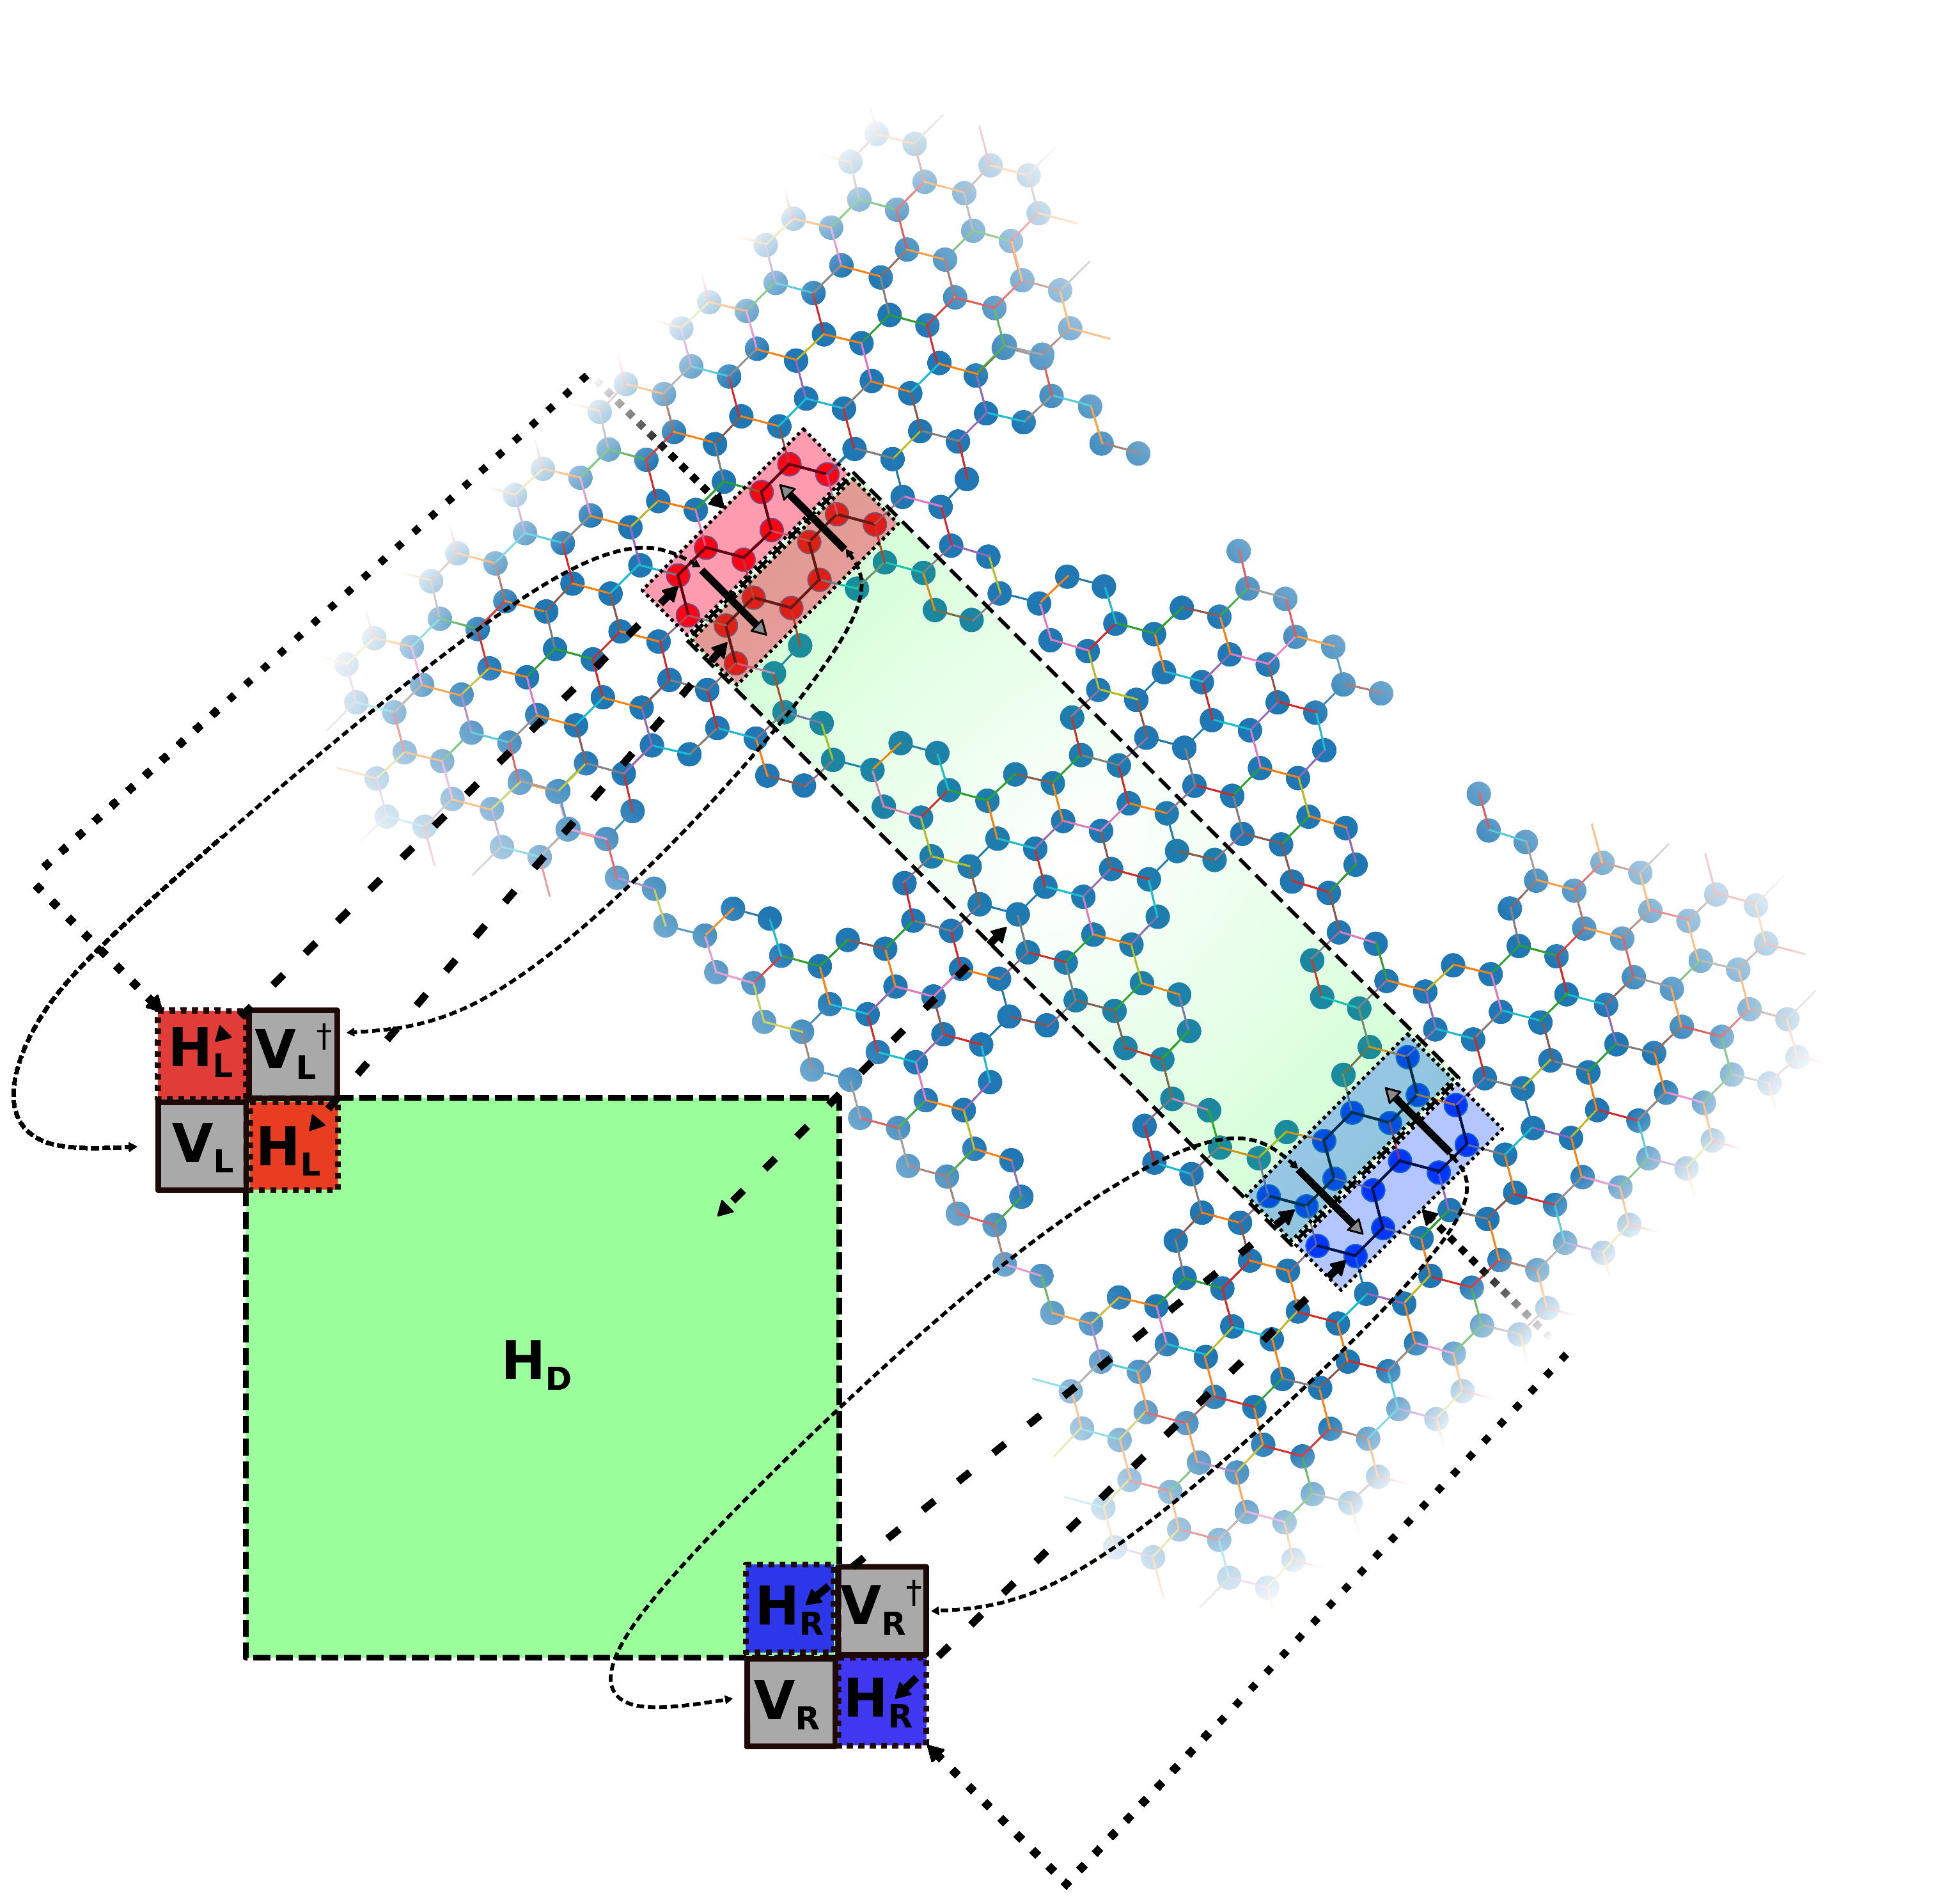
\includegraphics[width=0.9\textwidth]{Figures/illu.eps}
    \caption{Illustration showing how the different parts of the system are translated into matrix blocks. On the graphene the green box is the unit cell of the device. It includes one red and blue box which themselves are unit cells of the left and right contacts. These unit cells can be translated into Hamiltonian matrices \(\textbf{H}_D, \ \textbf{H}_L,\ \textbf{H}_R\) as illustrated. Note that because the first of the left and right unit cells (red and blue) are inside the device (green region), they can be picked out of \(\textbf{H}_D\) directly and so it is not necessary to make them from scratch. The two other unit cells lying outside the device region represents what could be an infinite contact region. The contact region is therefore potentially of an infinitely bigger dimension compared to the device region, however, by recursion, this region can be collapsed into a single Hamiltonian of same dimension as the one inside the device region. Finally the two fat black arrows (not dotted) on each side of the device represents the hopping between the device and contact region. Note that the direction of hopping corresponds to a specific hopping matrix. F.ex. left-to-right is the ordinary hopping matrix while right-to-left is its conjugate (for both left and right side of the device).}
    \label{systemillu}
\end{figure}
\subsubsection{Transmission in 1D a simple example}
As with the Recursion Routine, the development of this routine will be build up around a small system in order to make sure that the obtained results are as expected, thereafter generalising the routine to suit all kinds and sizes of system. First thing is to define the device in the same manner as \cref{systemillu} so that the device Hamiltonian \(\textbf{H}_D\) can be obtained through the already defined function \textit{Onsite}. The left and right Hamiltonian \(\textbf{H}_{L/R}\) are thus picked out as described in \cref{systemillu}. A smart function has been implemented in order to allow the user to choose the left and right contact cells using indices given to each atom in the system of choice (See \cref{basicstructurewithcontacts} for an example).
\begin{figure}
\begin{subfigure}[b]{0.4\textwidth}
		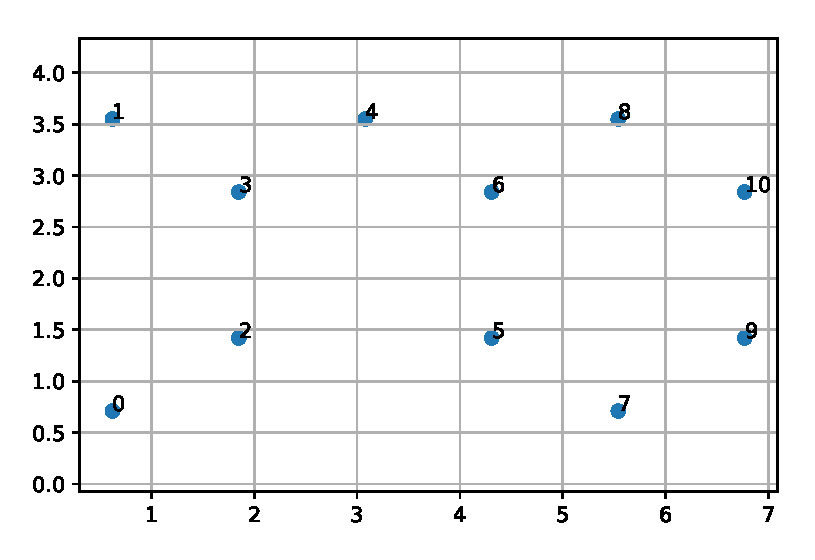
\includegraphics[width=\textwidth]{Figures/basicstructure.eps}
		\caption{The basic structure plotted with indices\vspace{\baselineskip}}
		\label{basicstructure}
	\end{subfigure}\vspace{2mm}
	~ %add desired spacing between images, e. g. ~, \quad, \qquad, \hfill etc.
	%(or a blank line to force the subfigure onto a new line)
	\begin{subfigure}[b]{0.4\textwidth}
		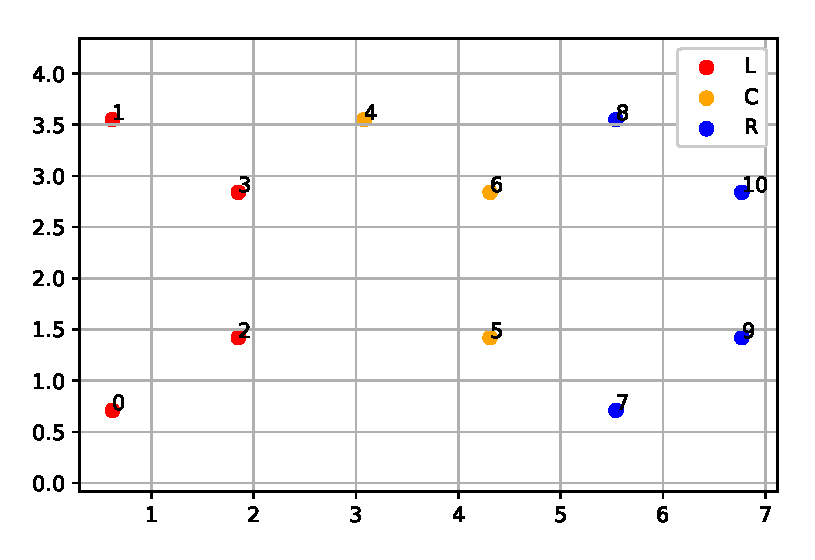
\includegraphics[width=\textwidth]{Figures/basicstructurewithcontacts.eps}
		\caption{The same structure now shown with indices marked red and blue as per users choice of contact atoms}
		\label{basicstructurewithcontacts}
	\end{subfigure}
	\caption{Figure showing the interface integrated into the script.}\label{interface}
\end{figure}
This allows the user to get the dimensions needed to define the left and right Hamiltonians so they can be picked out of the device Hamiltonian. From the left and right Hamiltonian the corresponding hopping matrices are defined using the \textit{Hop} function. Then the \textit{EnergyRecursion} is used to obtain the Green's function for the device. This function is a more elaborate version of the earlier mentioned \textit{RecursionRoutine}. It uses the old recursion routine to calculate the self energies for the left and right cells (\(\mathbf{\Sigma}_{L/R}\)) (see line 164-165 \cref{engrec}) and then uses those to calculate the device Green's function \(\textbf{G}_D\) as well as the left and right rate matrices \(\mathbf{\Gamma}_{L/R}\), using the equations \cref{rateeq}, \cref{devicegreens} (see \cref{engrec} line 176-179).\im{Listings/Functions.py}{156}{185}
\vspace{-1\baselineskip}
\captionof{listing}{lalala\label{engrec}}\vspace{\baselineskip}The output of the energy recursion function is the two rate matrices (left and right) as well as the device Green's function and as per \cref{transeq} the matrices needed for transmission have been obtained. As seen in \cref{transfunc} the transmission function \textit{Transmission} simply carries out the matrix product and subsequent trace of the resulting matrix and outputs a range of transmission probabilities which is then plotted against an energy range. Do mind that this is still just 1D in the sense that the transmission only moves in one direction. A plot of the transmission for such a simple 1D system (the one in \cref{basicstructure}) can be seen in \cref{alphatrans}.\im{Listings/Functions.py}{188}{195}
\vspace{-1\baselineskip}
\captionof{listing}{lalala\label{transfunc}}\vspace{\baselineskip}
\begin{figure}[ht]
    \centering
    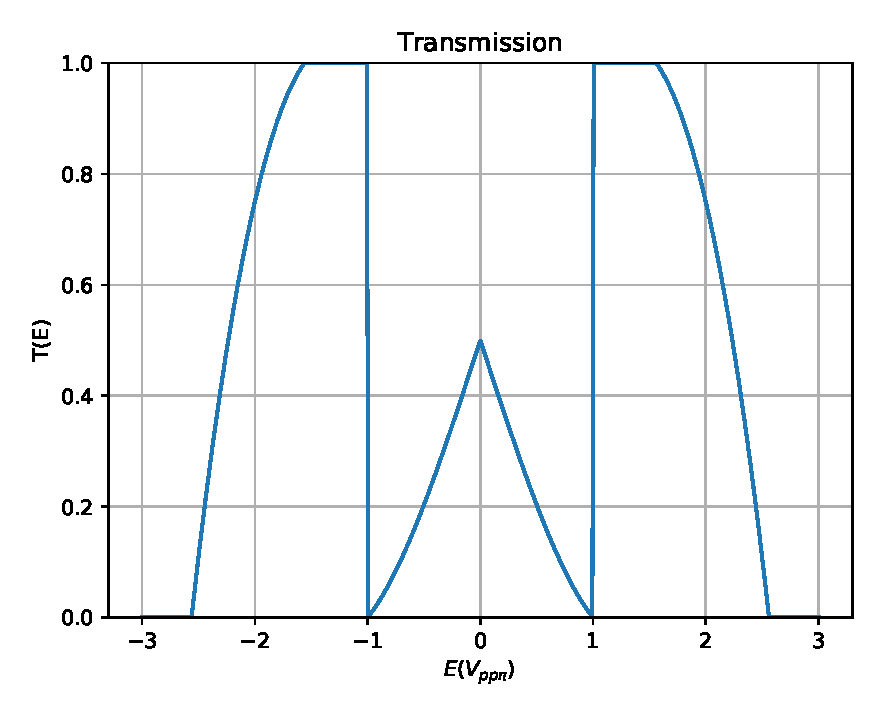
\includegraphics[width =0.5\textwidth]{Figures/alphaTE.eps}
    \caption{Transmission plot for the system in \cref{interface}}
    \label{alphatrans}
\end{figure}
\subsubsection{Development of transmission to 2D}
Lastly the transmission routine needs to be generalised so it can handle transport in two directions. The most convenient approach is to work with five real space unit cells as a starting point. One center cell, a right and a left cell representing the contacts and then two additional cells on the left and right, representing the rest of the contact region. This would be the minimum amount of cells needed to generalise the transmission. One might have more center cells if the structure changes from one of those cells to the other. First these five unit cells will be defined using already developed tools. Then a big Hamiltonian, including all coordinates from the five cells representing real space are created, again using existing functions. One could call this big Hamiltonian \(\textbf{H}_{\text{Bigreal}}(xyz_0,xyz_0)\). It is a function of two sets of identical coordinates, namely the ones used to create the Hamiltonian itself. This has also been the case for all previous calculations, but the following steps will make it clear why it is explicitly stated for this Hamiltonian. The left/right on-site Hamiltonians and hopping matrices can thus be picked out of \(\textbf{H}_{\text{Bigreal}}(xyz_0,xyz_0)\) as before to get the Green's functions, self energies for transmission in real space, just as in the previous section. But instead, before the Green's function, self energies and transmission is calculated, the left/right onsite-Hamiltonian as well as their hopping matrices are defined as functions of a variable \(k\) and the hopping will additionally have a phase added which depends on a variable \(q\). As an example the following is the equation for the full right side Hamiltonian using the right on-side Hamiltonian with its hopping matrices: \(\textbf{H}_R(k,q) = \textbf{V}_R(k)e^{iq}+\textbf{V}^{\dagger}_R(k)e^{-iq}+\textbf{h}_R(k)\). The \(k\) represents .... and the \(q\) represents ..... The next part is to obtain
the hop from \(\textbf{H}_{\text{Bigreal}}(xyz_0,xyz_0)\) to an equal cell in the other (transverse) direction, so that the transmission will become truly 2D. Firstly the hopping between \(\textbf{H}_{\text{Bigreal}}(xyz_0,xyz_0)\) and a transversely shifted Hamiltonian is defined as \(\textbf{W} = \textbf{H}_{\text{Bigtrans}}(xyz_0,xyz_1)\) (Here using \textbf{W} as not to confuse it with \textbf{V} which is hopping between cells in real space). Note that the index of one of the coordinate sets have changed to 1. This corresponds to a shift by the lattice vector going in the transverse direction to that of the transmission direction defined in 1D. With the hopping matrices for the transverse direction defined a Hamiltonian dependent on \(k\)-point values can be defined as:\begin{align}
    \textbf{H}(k) &= \textbf{h}+\textbf{W}e^{ik}+\textbf{W}^{\dagger}e^{-ik}\\
    &= \textbf{H}_{\text{Bigreal}}(xyz_0,xyz_0) + \textbf{H}_{\text{Bigtrans}}(xyz_0,xyz_1)e^{ik}+\textbf{H}_{\text{Bigtrans}}^{\dagger}(xyz_0,xyz_1)e^{-ik}
\end{align}
Now a Hamiltonian, dependent of a variable \(k\) has been defined, and thus it is now possible to get self energies, Green's functions that is \(k\)-dependent as well as a transmission (also \(k\)-dependent) which can be found for different \(k\)-points i.e. different points in the transverse direction (inverse space). This hereby concludes the all the initial effort to develop a code which can do calculations of different points of interest (Green's function plots, band structures and transmission) in a two dimensional material such as NPG. Following is a walk through as to how this last step has been implemented through code programming. 

\newpage
\begin{acknowledgments}
	The authors would like to thank...
\end{acknowledgments}
%End of text
% List of ToDos
%\listoftodos %Uncomment for list of todos
%Bibliography herunder:
%\newpage
\onecolumngrid
\bibliography{Bibliography}

\newpage
\listoffigures
\listoftables
\listoflistings
%\listoftodos
\newpage
 %Appendicer herunder:
% !TEX root = Main.tex
\appendix
\appendixpage
\addappheadtotoc
\section{Additional figures}\label{appfigs}
\begin{figure}[h]
	\centering
	\begin{subfigure}[b]{0.3\textwidth}
		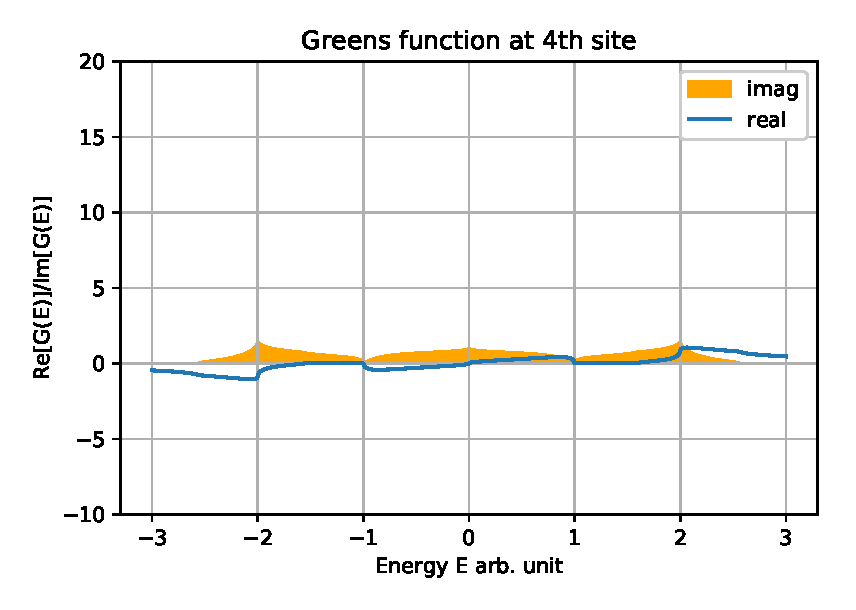
\includegraphics[width=\textwidth]{Figures/BetaimrealTE4.eps}
		\caption{Figure showing a plot of the Green's function at the 4th site}
		\label{4th}
	\end{subfigure}
	~ %add desired spacing between images, e. g. ~, \quad, \qquad, \hfill etc.
	%(or a blank line to force the subfigure onto a new line)
	\begin{subfigure}[b]{0.3\textwidth}
		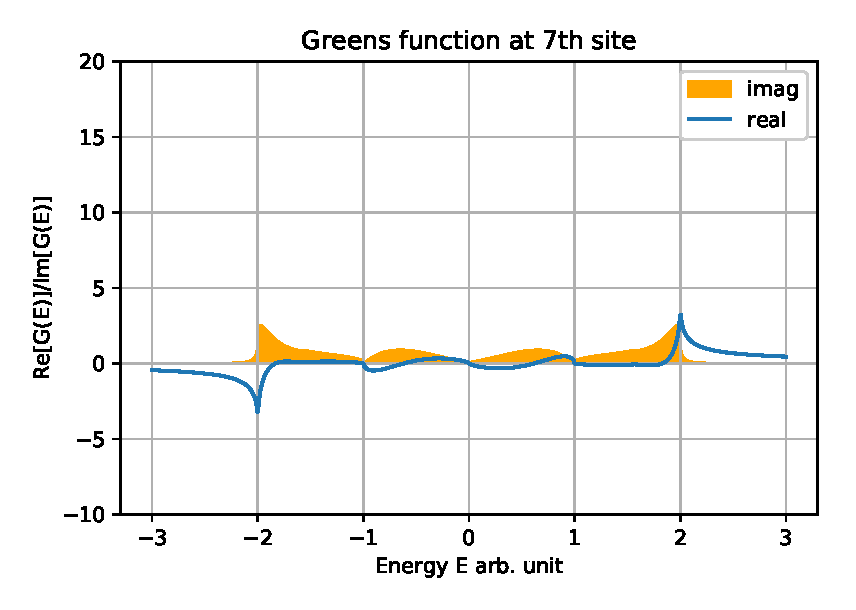
\includegraphics[width=\textwidth]{Figures/BetaimrealTE7.eps}
		\caption{Figure showing a plot of the Green's function at the 7th site}
		\label{7th}
	\end{subfigure}
	\caption{Two plots showing how the Green's function changes as the site is changed. The 4th and 7th sites are corresponding to atoms of those indices (4, 7) in \cref{pointplot}. Note how the LDOS changes (imaginary part) for the different sites.}\label{siteLDOSplot}
\end{figure}
\begin{figure}
	\centering
	\begin{subfigure}[b]{0.3\textwidth}
		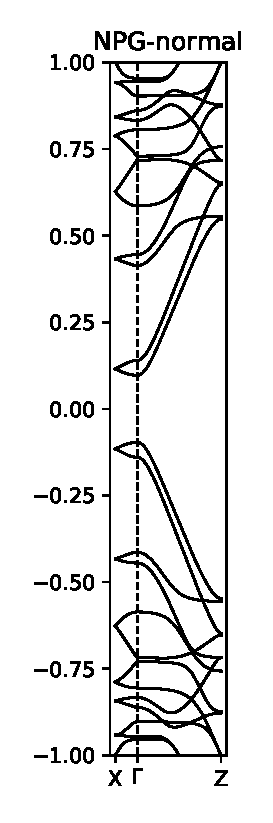
\includegraphics[width=\textwidth]{Figures/FabNPGBS.eps}
		\caption{Plot showing the band structure in the energy range \SI{-1.5}{\electronvolt} to \SI{1.5}{\electronvolt} for NPG with normal bridges between symmetry points \(X\) and \(Y\) with respect to \(\Gamma\)}
		\label{Fabbs}
	\end{subfigure}
	~ %add desired spacing between images, e. g. ~, \quad, \qquad, \hfill etc.
	%(or a blank line to force the subfigure onto a new line)
	\begin{subfigure}[b]{0.3\textwidth}
		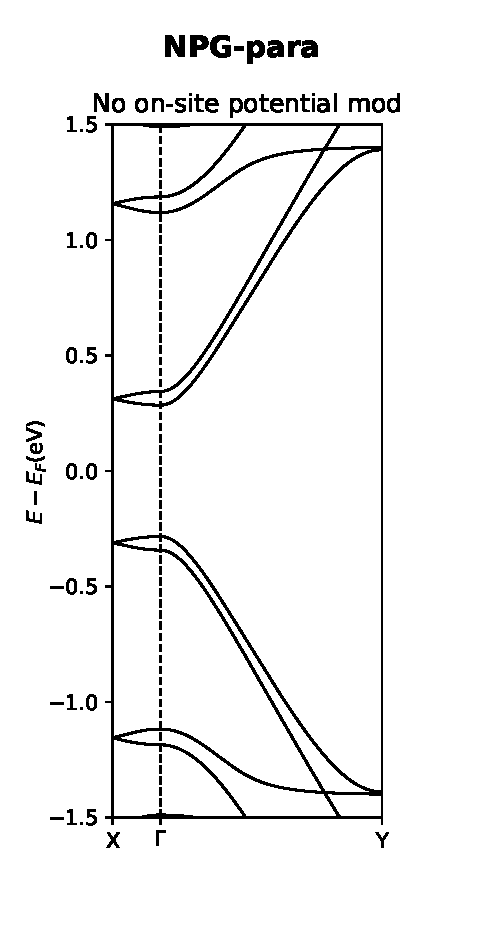
\includegraphics[width=\textwidth]{Figures/paraNPGBS.eps}
		\caption{Plot showing the band structure in the energy range \SI{-1.5}{\electronvolt} to \SI{1.5}{\electronvolt} for NPG with para bridges between symmetry points \(X\) and \(Y\) with respect to \(\Gamma\)}
		\label{parabs}
	\end{subfigure}
	~ %add desired spacing between images, e. g. ~, \quad, \qquad, \hfill etc.
	%(or a blank line to force the subfigure onto a new line)
	\begin{subfigure}[b]{0.3\textwidth}
		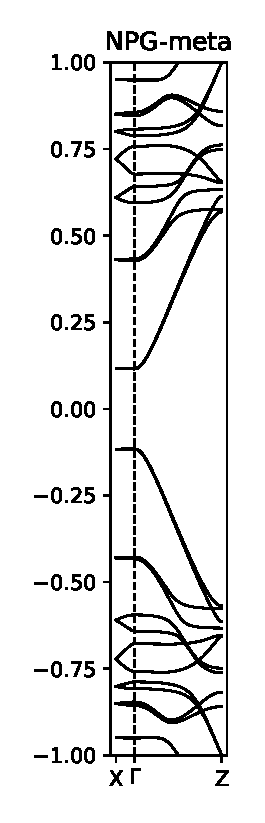
\includegraphics[width=\textwidth]{Figures/metaNPGBS.eps}
		\caption{Plot showing the band structure in the energy range \SI{-1.5}{\electronvolt} to \SI{1.5}{\electronvolt} for NPG with meta bridges between symmetry points \(X\) and \(Y\) with respect to \(\Gamma\)}
		\label{metabs}
	\end{subfigure}
	\caption{Figure showing para, meta and normal NPG band structures}\label{allbands}
\end{figure}
\im{Listings/Functions.py}{41}{47}
\vspace{-1\baselineskip}
\captionof{listing}{Function creating the hopping matrices between two sets of coordinates \label{hopfunc}}\vspace{\baselineskip}

\begin{figure}
	\centering
	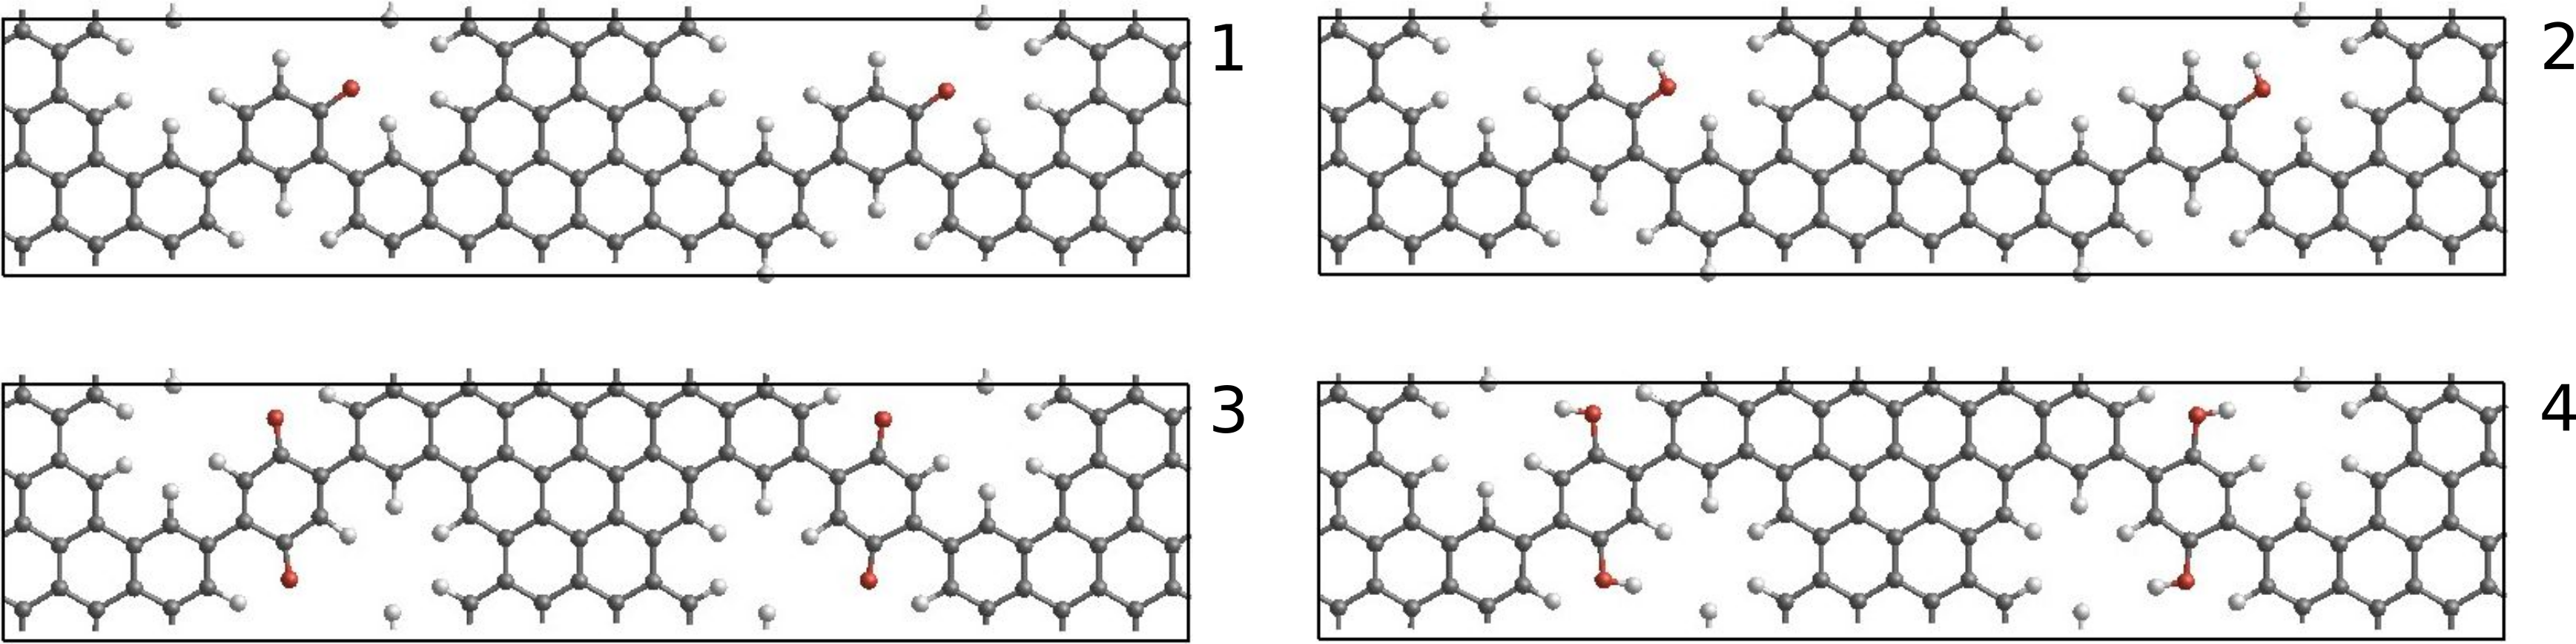
\includegraphics[width=\textwidth]{Figures/Structures.png}
	\caption{Figure showing all the structures stated in \cref{testtable}.}
	\label{Strucow}
\end{figure}

\im{Listings/Functions.py}{245}{252}
\vspace{-1\baselineskip}
\captionof{listing}{Code piece showing how the periodic Hamiltonian, shifted in the transverse direction i created using the given unit vector in the y direction.}{\label{periodichamilcode}}\vspace{\baselineskip}

\im{Listings/Functions.py}{234}{242}
\vspace{-1\baselineskip}
\captionof{listing}{Code piece showing how the transmission per energy point, using equation \cref{}.}{\label{transmissioncode}}\vspace{\baselineskip}

% \section{Project overview}
% A Gantt chart is provided on the next page. \textbf{Not Updated.}
% \newpage
% \begin{turnpage}
% \setcounter{myWeekNum}{6}
% \ganttset{%
% 	calendar week text={\myWeek{}}%
% }
% \begin{figure}\vspace{-10mm}
% \begin{ganttchart}[
% 		hgrid,
% 		vgrid={*{6}{draw=none}, dotted},
% 		x unit=.15cm,
% 		%	y unit title=.6cm,
% 		%	y unit chart=.6cm,
% 		inline,
% 		milestone inline label node/.append style={left=5mm},
% 		milestone/.append style={xscale=3},
% 		time slot format=isodate,
% 		time slot format/start date=2019-02-04
% 	]{2019-02-04}{2019-05-31}
% 	\gantttitlecalendar{year, month=shortname, week}\\
% 	\ganttgroup{Report writing}{2019-02-25}{2019-05-31}\\
% 	\ganttgroup[inline = false]{Course 33442}{2019-02-04}{2019-03-31}\\
% 	\ganttbar{Ch. 1 \& 2}{2019-02-04}{2019-02-17}\\
% 	\ganttlinkedbar[link bulge=2]{Ch. 3}{2019-02-18}{2019-02-24}\\
% 	\ganttlinkedbar[link bulge=2,bar inline label node/.style={right=15pt}]{Ch. 4 \& 5}{2019-02-25}{2019-03-03}\\
% 	\ganttgroup[inline = false]{Python code}{2019-03-04}{2019-03-31}\\
% 	\ganttbar{Py TB scripts}{2019-02-18}{2019-03-17}\\
% 	\ganttlinkedbar[link bulge=2, bar inline label node/.style={right=45pt}]{Small NPG systems simulations}{2019-03-10}{2019-03-31}\\
% 	\ganttmilestone{Proof of Concept with Python}{2019-03-31}\\
% 	\ganttgroup[inline = false]{Large scale TB}{2019-04-01}{2019-04-28}\\
% 	\ganttbar[bar inline label node/.style={left=10pt}]{SISL \& TBtrans tutorial}{2019-04-01}{2019-04-05}\\
% 	\ganttlinkedbar[link bulge=2, bar inline label node/.style={right=50pt}]{Setup NPG variations}{2019-04-06}{2019-04-28}\\
% 	\ganttgroup[inline = false]{Generate data}{2019-04-28}{2019-05-31}\\
% 	\ganttmilestone{Hand in report}{2019-05-31}
% \end{ganttchart}
% \end{figure}
% \end{turnpage}
% \clearpage
% \global\pdfpageattr\expandafter{\the\pdfpageattr/Rotate 90}

\end{document}
